%++++++++++++++++++++++++++++++++++++++++
% Don't modify this section unless you know what you're doing!
\documentclass[letterpaper,10pt]{article}
\usepackage{tabularx} % extra features for tabular environment
\usepackage{textcomp}
\usepackage{gensymb}
\usepackage{amsmath}  % improve math presentation
\usepackage{graphicx} % takes care of graphic including machinery
\usepackage{subfig}
\usepackage{wrapfig}
\usepackage{xcolor}
\usepackage{rotating}
\usepackage[margin=1in,letterpaper]{geometry} % decreases margins
\usepackage{setspace}
\usepackage{cite} % takes care of citations
\usepackage[final]{hyperref} % adds hyper links inside the generated pdf file
\hypersetup{
	colorlinks=true,       % false: boxed links; true: colored links
	linkcolor=blue,        % color of internal links
	citecolor=blue,        % color of links to bibliography
	filecolor=magenta,     % color of file links
	urlcolor=blue         
}
%++++++++++++++++++++++++++++++++++++++++
\graphicspath{{/Users/clay/Documents/research/jgr20/manuscript/plots/}}

\begin{document}
	
\doublespacing

%\title{The Effect of Roughness on the Elasticity and Permeability of Fractured Media}
%\author{C. Wood, B. Madera, P. Shokouhi, J. Jin, J. Rivi\`{e}re, D. Elsworth, C. Marone}
%%\date{\today}
%\maketitle


\section{Possible Titles}
\begin{flushleft}
	\begin{Large}
		\textbf{Elastodynamic and hydraulic properties of fractured and sheared rock: An experimental investigation 
			\linebreak \linebreak \linebreak
			\textcolor{red}{Imaging elastodynamic and hydraulic properties of in-situ fractured rock: An experimental investigation exploring effects of dynamic stressing and shearing}}
	\end{Large}
\end{flushleft}


\section{Abstract}
We describe laboratory work to elucidate the relationship between nonlinear elasticity and
permeability of fractured media subjected to local stress perturbations in relation to fracture
roughness and aperture distribution. This study is part of an effort to image fluid pathways and
fracture properties using locally induced seismicity, associated with fluid injection. Experiments were conducted in which intact L-shaped Westerly Granite samples were fractured in-situ tri-axial conditions while forcing deionized water through the subsequent fracture interfaces. After in-situ fracture, we imposed oscillations of the applied Normal stress and pore pressure with amplitudes ranging from 0.2 to 1 MPa and frequencies from 0.1 to 10 Hz. During these dynamic perturbations an array of ultrasonic transducers (PZTs) continuously generated and transmitted p-wave pulses to monitor the elastic response of the granite samples. We interpret the relative change in p-wave velocities to be an analog for the elastic non-linearity and relate it to the permeability of the fractured media. The roughness of the fracture interfaces is altered during experiments by shearing the L-shaped samples and then allowing the interface to age before applying dynamic stressing. We observe changes in the permeability and stiffness of the fracture during the dynamic perturbations and also with the shearing history, changing roughness, of the Westerly Granite samples.


\section{Introduction}
%\textcolor{red}{As you yourself have noted, this is very similar to GRL’s introduction and needs to be re-written.}\\
%\textcolor{red}{We will need to include a paragraph (w relevant literature) discussing how shearing changes nonlinearity.}\\

\paragraph{} Dynamic stresses associated with energy production and waste water sequestration (injection, pumping, and transport of supercritical $H_{2}O$--$CO_{2}$ fluids) are particularly concerning as they are known to induce seismicty [Healy et al., 1968; Raleigh et al., 1976; Simpson et al., 1988; Sminchak and Gupta, 2003; McNamara et al., 2015; McGarr et al., 2015; Walsh and Zoback, 2015]. \cite{rtmQ,migExt}

\paragraph{} Though dynamic stressing could be beneficial for enhanced permeability, it presents a significant risk associated with fault reactivation, reservoir seal damage, and accelerated deformation. Therefore, it is important to understand how fluid injection influences the hydromechanical properties of rocks and fractures. We have performed careful laboratory experiments to investigate the connection between fluid flow and elastic nonlinearity (i.e. stress is not proportional to strain) of fractured media.

\paragraph{} Dynamic stressing of the local subsurface associated with seismicity, drilling, hydraulic injection cause transient changes in permeability. These perturbations cause significant changes in the local stress field and consequently the poromechanical properties of the local subsurface. Empirical evidence from the field and laboratory show that earthquakes and subsequent seismic waves cause transient changes in rock stiffness in the proximity of faults. Specifically, measurements of a sudden decrease in seismic wave velocity from co-seismic softening and a post-seismic relaxation of the rock stiffness, a logarithmic recovery in time. Scaling down to laboratory studies, it has been shown that by using dynamic acousto-elastic testing, ultrasonic wave velocity (analog for field-scale seismometers) recorded decreased during dynamic stressing and then recovered after dynamic stressing ended with a logarithmic form. Dynamic perturbations with strain on the order of $10^{-6}$ cause a transient decrease in stiffness in nonlinear elastic materials. 
%\textit{It would be nice to mention any studies b/w lab- and field-scale.} 

\paragraph{} Anthropogenic activities on the field-scale such as drilling, wastewater storage, hydraulic fracturing result in considerable deformation of reservoir rocks. Changing the hydromechanical properties by dynamic stressing from fluid injection are likely to present hazards in the form of fault reactivation and reservoir seal damage. Evidence of this type of stressing inducing regional seismicity is rich and numerous (\textit{more details and citations}). Despite the hazards, dynamic stressing of the subsurface may result in enhanced permeability, consequently greater energy recovery. 
Seismic and anthropogenic sources of dynamic perturbation both change rock stiffness and permeability in similar ways, which suggests there is a physical mechanism that relates the nonlinear stiffness and poromechanical properties of fractured rock.

\paragraph{} Nonlinear response is sensitive to many fracture properties: geometry, flow pathways, asperity compliance, and friction. Currently, literature for investigating the relationship b/w elastodynamic and poromechanical and subsequent recovery is quite limited. We present the results from sophisticated well-controlled laboratory experiments in which we combine the analysis of nonlinear elastodynamic and hydraulic data. 

\paragraph{} It is expected that the nonlinear behavior of rocks is sensitive to fine features such as fracture aperture (i.e. flow pathways, asperity stiffness). In order to fully under-stand the ramifications of dynamic stressing in the subsurface, we need elucidate the relationship between the elastodynamic and hydro-mechanical properties of fractured rocks. 

%\graphicspath{{./plots/}}


\section{Experimental Setup}
\label{sec:experimnt_setup}

\paragraph{} We conducted sophisticated experiments in which samples were loaded under triaxial conditions inside a pressure vessel and fractured in-situ to simultaneous measure flow rate and elastic properties. Westerly granite samples were prepared by cutting them into L-shape blocks (69 x 45 50 x 26 mm, Figure \ref{fig:samplesetup}) with 3 mm deep notches on the top and bottom to ensure reproducibility of planar fracture propagation. The L-shape is used for maintaining constant nominal contact area during fracture and shear. The samples were saturated in deionized water and then placed between steel forcing blocks that have embedded piezoelectric transducers. The P-polarized lead-zirconate transducers (PZTs) of company APC International Ltd. are 6.5 mm in diameter, with a center frequency of 500 kHz and the spacing between the steel loading platen and the PZTs is 4mm. The shorter forcing block additionally contains internal conduits to provide fluid flow along the fracture plane. Deionized water was pumped through these narrow channels (45 x 1 mm) and covered by sintered porous fits and fed by five 1.6 mm diameter holes. Sintered porous frits (permeability ~ $10^{-14}$ $m^2$) are press-fit into cavities within the short forcing block to allow homogenous distribution of fluid. After securing this Single Direct Shear (SDS) configuration, it was sealed inside a latex jacket to separate confining and pore fluids. Fully prepared and jacketed samples were fitted inside a pressure vessel within a biaxial loading apparatus.

\paragraph{} The Biax consists of two hydraulic pistons capable of applying vertical and horizontal loads in displacement or load control. Forces are measured using custom-built, beryllium-copper strain-gauge load cells mounted on each loading piston. The load cells have an amplified output of ±5 V with an accuracy of ±5 N and are calibrated with a Morehouse proving-ring. Displacements are measured with direct-current displacement transducers (DCDT), with an accuracy of $\pm$ 0.1 $\mu m$. The confining fluid, a food-grade heat transfer oil (XCELTHERM 600, Radco Industries), in the sealed pressure vessel is pressurized to create a true-triaxial stress conditions. A linear variable differential transformer was attached to the outside of the sample, inside the pressure vessel, to accurately ($\pm 0.1\ \mu m$) measure the fracture displacement. Pressure intensifiers fitted with LVDTs and pressure transducers were used to control the confining pressure and the internal upstream and downstream pressures. 

\paragraph{} Each axis of loading is independently servo-controlled and all stresses, strains, fluid pressures and fluid volumes were recorded with $\pm10$ V, 16-channel 24-bit analog-to-digital converter at 10 kHz and averaged to sampling rates of 100 Hz or 1 kHz. Fracture permeability was measured using upstream and downstream pore-pressure intensifiers. Active ultrasonic data were recorded using a Vantage\textsuperscript{TM}\ Research Ultrasound (Verasonics) system. We use broadband (~0.02-2 MHz) PZTs (APC International Ltd. 6.35 diameter compressional crystals), which were successively pulsed every 1 ms on the transmitting side and the recording rate at the receiver side was 25 MHz. The input signal is a half sine with a frequency of 500 kHz. Also, a pulse from the Verasonics system accompanied the PZT excitation and is recorded by the 24-bit analog-to-digital data acquisition system. This allows us to sync the “ultrasonic” to “poro-mechanical” data and then analyzed to measure changes in the permeability and elasticity of the fractured rock samples, explained more fully in the signal analysis procedure.
  
\paragraph{} Before commencing each experiment, the samples were installed in the pressure vessel and then the vessel was sealed and then filled with confining fluid. A horizontal load of 20 MPa was applied and then the confining fluid pressure was slowly increased to 15 MPa; it is important to monitor the integrity sample jacket seal during this step. Next, we applied a pore pressure differential: inlet ($P_{pA}$ = 4 MPa) and outlet ($P_{pB}$ = 2 MPa). At this point there was no flow because Westerly granite matrix permeability is very low ($< 10^{-20}\ m^2$) and the confining fluid pressure is greater than the pore pressure (there was no flow around the sample). After establishing all loads and pore pressure, the ultrasonic data acquisition Once all fluid pressures and solid stresses were applied, the ultrasonic data acquisition system (Verasonics\textsuperscript{\textregistered}) was started. The sample was then fractured in situ by increasing the shear stress at constant normal stress while making continuous measurements of fluid flow and ultrasonic properties. After locking the vertical piston (no displacement allowed), we executed the dynamic stressing protocol illustrated in Figure 2a.

\paragraph{} After executing the normal stress and pore pressure oscillation protocol, the fractured sample was sheared twice in 4 mm increments (for a total of 8 mm). During the shearing phases of the experiment acoustic emissions (AEs) were monitored (passive source recording). Subsequent to shearing the dynamic stressing protocol was repeated. We incorporate shearing in this investigation to determine its influence on the nonlinearity measurements of the fracture. The fracture aperture is changed through shear, in effect, modeling the complexity of fractured subsurface rock. 

\newpage

\begin{figure*}[ht] 
	% read manual to see what [ht] means and for other possible options
	\centering 
	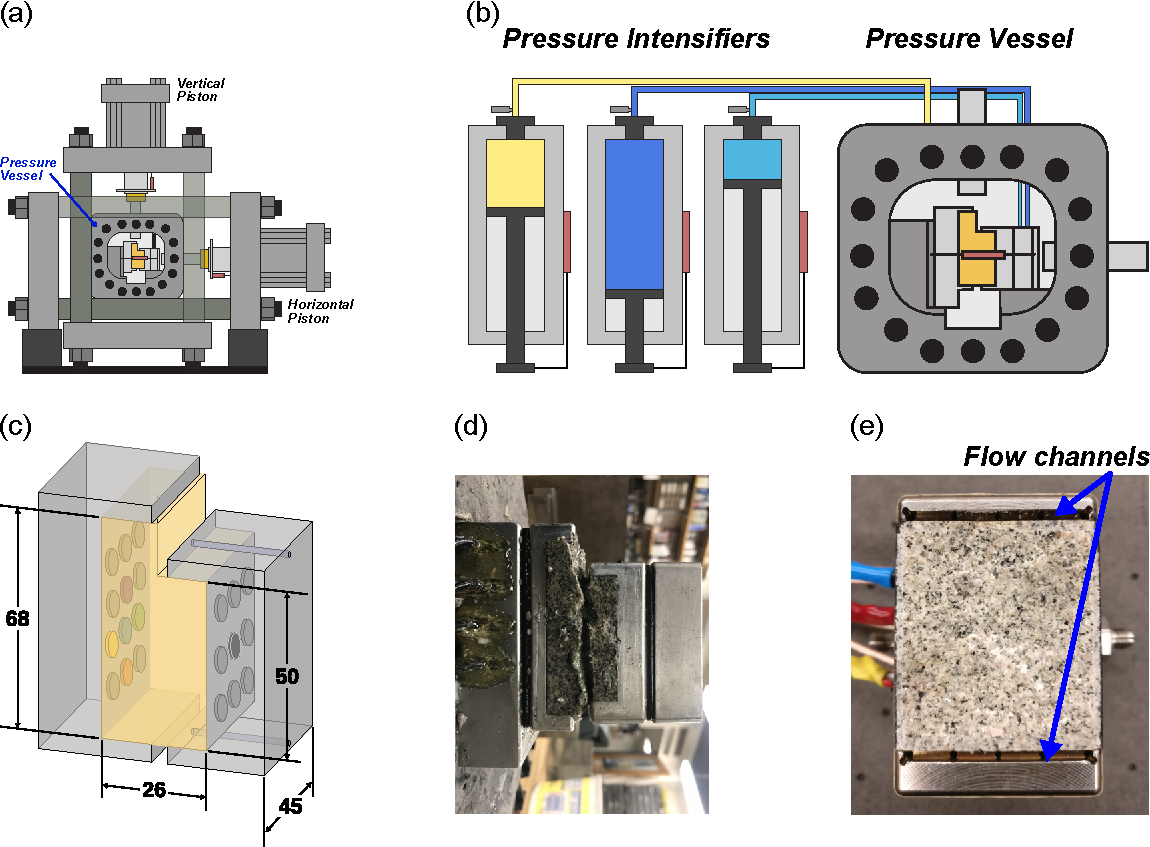
\includegraphics[width=0.9 \columnwidth]{experimental_configuration}
	\caption[]{(a) The experiments were conducted in the Penn State Rock and Sediment Mechanics laboratory using the Biaxial Deformation Apparatus (Biax). The Biax has servo-controlled vertical and horizontal pistons and a 10 kHz 24-bit analog to digital data recorder. (b) A pressure vessel was inserted in the Biax and connected to the pressure intensifiers, which control the confining ($P_C$), and sample ($P_{PA}$ and $P_{PB}$ ) fluid pressures. (c) The Westerly granite sample is machine cut into a L-shape and placed between the two loading platens. These loading platens are embedded with piezoelectric transducers (p-polarized) and contain fluid ports for the inlet and outlet flow. The shorter forcing block additionally contains internal conduits to provide fluid flow along the fracture plane. Deionized water was pumped through these narrow channels (45 x 1 mm) and covered by sintered porous fits and fed by five 1.6 mm diameter holes. Sintered porous frits (permeability $\sim 10^{-14}\ m^2$) are press-fit into cavities within the short forcing block to allow homogeneous distribution of fluid. After securing this Single Direct Shear (SDS) configuration, it was sealed inside a latex jacket to separate confining and pore fluids. (d) A photo of the sample after experimentation highlights the degree of roughness of the in-situ fracture.}
	\label{fig:samplesetup} 
\end{figure*}

\newpage

\begin{figure*}[ht]
	\centering
	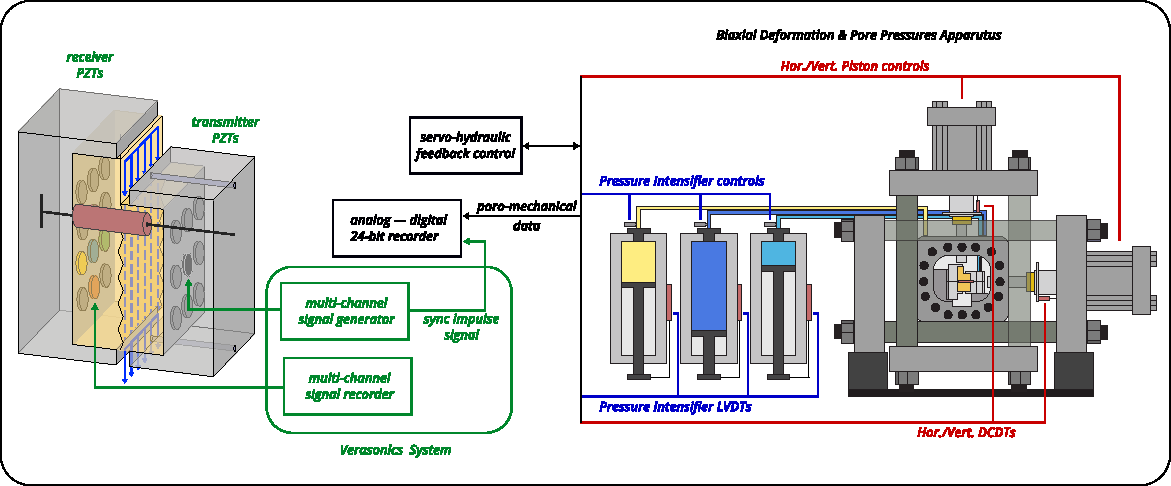
\includegraphics[width=0.9 \columnwidth]{exp_daq_v1}
	\caption[]{Schematic of the single direct shear configuration with the block diagram showing the main features of the data acquisition system for both the poro-mechanical and ultrasonic data. The Biax consists of two hydraulic pistons capable of applying vertical and horizontal loads in displacement or load control. Forces are measured using custom-built, beryllium-copper strain-gauge load cells mounted on each loading piston. The load cells have an amplified output of 5 V with an accuracy of 5 N and are calibrated with a Morehouse proving-ring. Displacements are measured with direct-current displacement transducers (DCDT), with an accuracy of $\pm 0.1 \mu m$. Each axis of loading is independently servo-controlled and all stresses, strains, fluid pressures and fluid volumes were recorded with 10 V, 16-channel 24-bit analog-to-digital converter at 10 kHz and averaged to sampling rates of 100 Hz or 1 kHz. Fracture permeability was measured using upstream and downstream pore-pressure intensifiers. Active ultrasonic data were recorded using a Vantage TM Research Ultrasound (Verasonics) system. We use broadband (0.02-2 MHz) PZTs (APC International Ltd. 6.35 mm diameter compressional crystals), which were successively pulsed every 1 ms on the transmitting side and the recording rate at the receiver side was 25 MHz. The input signal is a half sine with a frequency of 500 kHz. Also, a pulse from the Verasonics system accompanied the PZT excitation and is recorded by the 24-bit analog-to-digital data acquisition system. This allows us to sync the ultrasonic to poro-mechanical data and then analyzed to measure changes in the permeability and elasticity of the fractured rock samples, explained more fully in the signal analysis procedure.}
	\label{fig:data_aq}
\end{figure*}

\newpage


\subsection{Experimental Procedure}
\paragraph{}
Each experiment commenced with extensive sample preparation: in which the Westerly granite was cut and notched, sealed in a latex jacket, and then placed inside the pressure vessel (see Section \ref{sec:experimnt_setup} for details). After sealing the pressure vessel and loading the sample, inlet and outlet flow were pressurized to 4 MPa and 2MPa, respectively. At this stage there was no flow because Westerly granite matrix permeability is very low ($< 10^{-20}\ m^2$ ) and the confining fluid pressure (around the jacketed sample) is much larger than the pore pressure, preventing flow of water around the sample.
A shear load was then applied with the vertical piston in displacement mode at a constant 10 $\mu m/s$, fracturing in-situ after reaching a critical stress of $ \approx $60 MPa, and then locked the vertical piston. During fracture fluid flow and acoustic emissions were measured, but these results are not included in this paper. Next, the dynamic stressing protocol was implemented in which the normal stress and pore pressure were modulated. Normal stress oscillations were applied by oscillating the horizontal piston of the load frame at prescribed amplitudes (0.2 to 3 MPa) and frequencies (0.1, 1, 10, 40 Hz). Pore pressure oscillations were achieved by oscillating $P_{PA}$ while holding $P_{PB}$ constant at amplitudes of 0.2 to 3 MPa and frequencies of 0.1, 1, 10 Hz. Multiple sets of normal stress and pore pressure oscillations of varying amplitudes and frequencies were applied to investigate: (1) repeatability and direct comparison between the two modulated stresses and (2) amplitude and frequency dependencies of the measured response. Post-fracture dynamic stressing is plotted in Figure \ref{fig:exp_seq}d (highlighted in yellow) and shows the normal stress (red) and pore pressure (blue) oscillations; note that line thickness correlates with oscillation frequency. 
To investigate the effect of fracture aperture on elastic nonlinearity and permeability, the sample was sheared in two 4 mm, (held at $ \sigma_{NS} $ = 20 MPa) stages. After each shearing stage the oscillation protocol was applied to the sample. Initially,the in-situ fracture was quite rough, but the effect of shear reduces and changes this roughness; the old contacts were broken and new contacts formed, changing the extent to which the two halves of the fracture were mated. This allows for investigation of how fracture aperture is related to the elasto-dyamic and hydromechanical properties. 

\newpage


\begin{figure*}[ht]
	\centering
	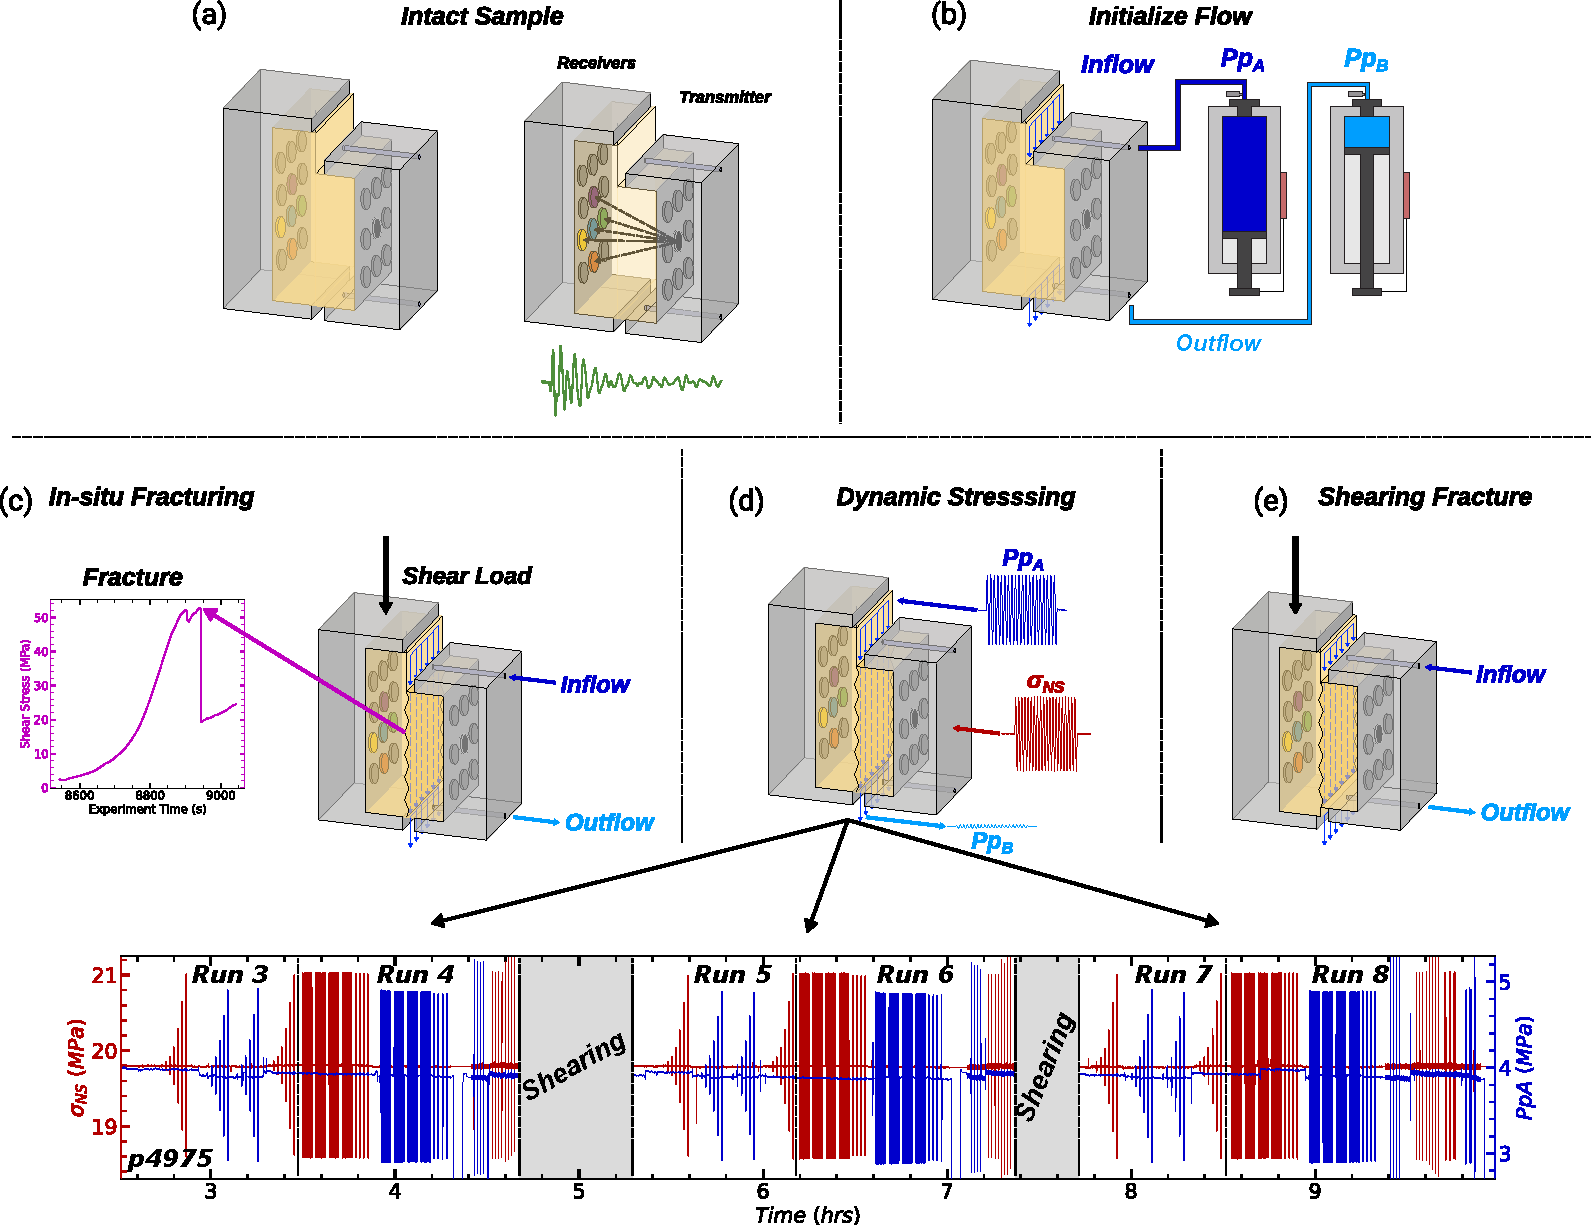
\includegraphics[width=0.99\columnwidth]{exp_sequence_v2}
	\caption[]{(a) Intact Westerly granite sample cartoon, showing dimensions and approximate transmitter - receiver ray paths. 
		(b) Next, we applied a pore pressure differential: inlet ($P_{PA}$ = 4 MPa) and outlet ($P_{PB}$ = 2 MPa). 
		(c) The shear stress was loaded at a constant rate of 10 $\mu m/s$ until reaching the critical shear stress at $ \approx $60 MPa. 
		(d) Cartoon showing the oscillation protocol applied to the freshly fractured sample. Multiple sets of $P_{P}$ and $ \sigma_{NS} $ oscillations of varying amplitude (up to about $ \pm $ 1 MPa) and frequency (0.1, 1, 10 and 40 Hz) were applied. 
		(e) The sample was sheared in two additional increments of 4mm, each followed by the dynamic stressing protocol.}
	\label{fig:exp_seq}
\end{figure*}


\newpage

\subsection{Dynamic Effective Stress Perturbations}
The fractured samples were dynamically perturbed via pore pressure ($P_P$) and normal stress ($\sigma_{n}$) oscillations. Following the procedure described by Candela et al., 2015, pore pressure oscillations were achieved by oscillating $P_{PA}$ while holding $P_{PB}$ constant. Conversely, normal stress oscillations were
applied by oscillating the horizontal piston of the load frame at prescribed amplitude and frequency. 
As depicted in Figure 2a, multiple sets of Pp and $\sigma_n$ oscillations of varying amplitude (up to about $\pm$ MPa) and frequency (0.1, 1, 10 and 40 Hz) were applied to investigate the repeatability as well as amplitude and frequency dependencies of the measured response. Similar parameters were used for $P_P$ and $\sigma_{n}$ oscillation sets in order to apply similar effective stress perturbations and allow making comparisons between $P_P$ and $\sigma_{n}$ stimulations.


\subsection{Permeability Measurements}
\paragraph{} We measured flow rates independently at the inlet ($Q_A$) and outlet ($Q_B$) using the outputs of LVDTs on the pressure intensifiers. After verifying the steady state flow condition ($Q_{A} - Q_{B}  \leq 5 \% $), Darcy’s law was
used to calculate permeability k: 
\begin{equation} \label{eq:perm}
k = \frac{\mu L}{S} \frac{Q}{\Delta P_P}
\end{equation}
where $Q = \frac{1}{2} (Q_A + Q_B )$ is the average flow rate ($\frac{m^3}{s}$), $\mu$ is the fluid viscosity ($10^{-3} Pa\cdot s$) at 20\textdegree\ C, $L$ is the flow path given by the length of the sample (50 mm) and $S$ is the cross section perpendicular to the flow path (45 x 26 $mm^2$).
\paragraph{} Specifically, k is the bulk permeability, that is, the permeability of the surrounding rock matrix (on order of $10^{-21} m^2$) and of the fracture [Zhang et al., 2017; Ishibashi et al., 2018]. Alternative calculations of permeability are valid [Zhang et al., 2017; Ishibashi et al., 2018], however we are interested in relative changes in permeability in response to dynamic stressing, so the absolute value of the permeability is not necessary to quantify.


\subsection{Ultrasonic Measurements: Active Source}
Ultrasonic waves transmitted through the fracture were recorded continuously in each experiment. Half-cycle sinusoidal pulses with an amplitude of 40 V and center frequency of 500 kHz were emitted consecutively from each transmitting transducer (9 piezoelectric discs arranged in a 3 x 3 matrix embedded within the right-hand loading block in Figure 1b) with a pulse repetition frequency (PRF) of 100 Hz or 1000 Hz during the low and high frequency ($\geq 10$ Hz) stress oscillations, respectively. The waveforms were amplified ($\sim 40$ dB) and recorded for all the receiving transducers (12 piezoelectric discs arranged in a 4 x 3 matrix embedded within the left-hand loading block in Figure 1b). We activated up to the full array of 9 transmitter and 12 receivers. 

\newpage

\begin{figure*}[ht]
	\centering
	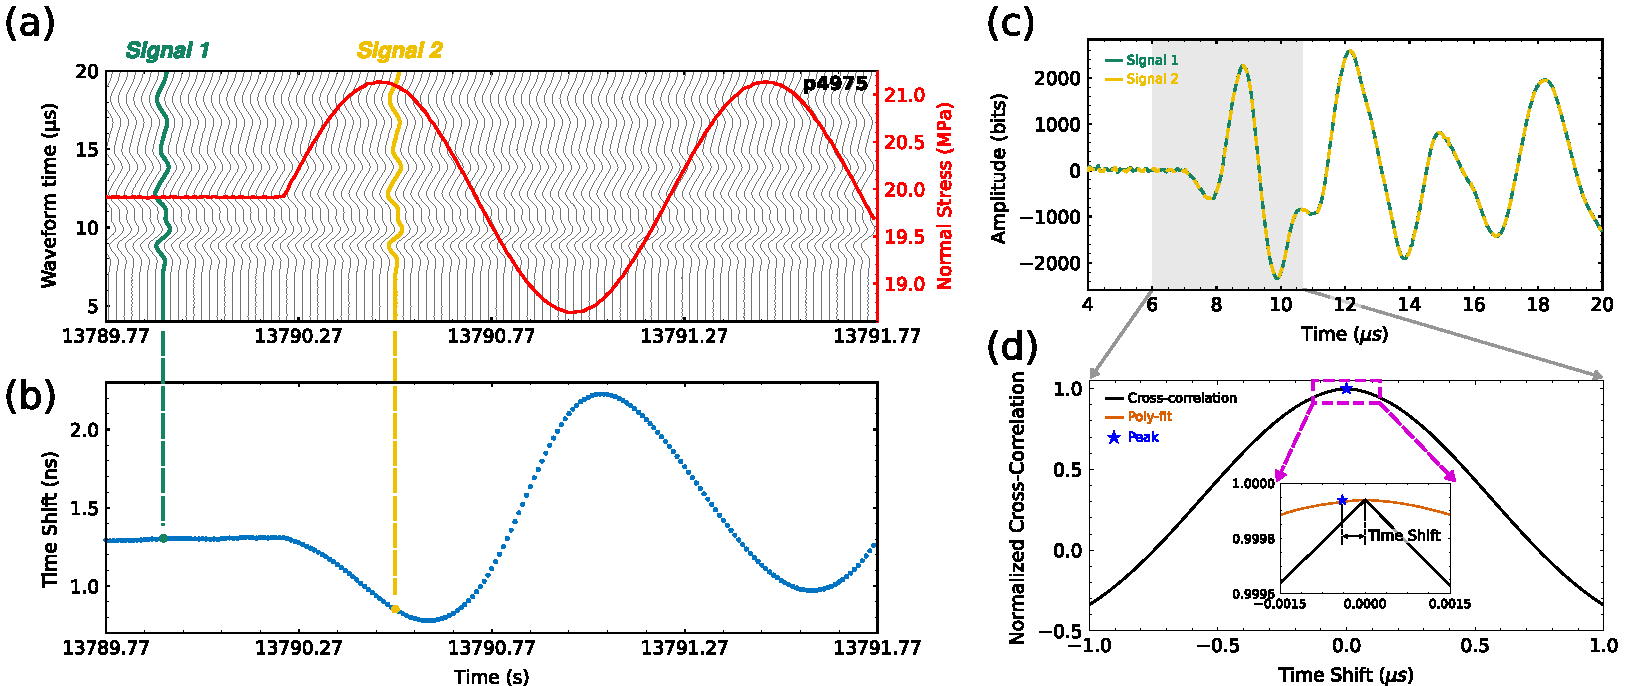
\includegraphics[width=0.9 \columnwidth]{xcor_fig_v3}
	\caption[]{(a) Excerpt from run4 of experiment p4966 shows part of a 1 Hz, 1 MPa normal stress oscillation (red) and the concurrent raw ultrasonic waveforms (grey). The number of waveforms in the waterfall plot has been decimated version for clarity. (b) Time shift was calculated by cross-correlating the waveforms to a reference waveform. (c) An example of a reference, unperturbed, waveform (green) and perturbed waveform (dashed yellow) highlights
		the similarity. (d) The maximum linear correlation between the reference and perturbed waveforms from cross-correlation is used to determine the time shift. The inset shows improvement of time shift calculations with a 2nd order polynomial fitting procedure.}
	\label{fig:xcor_poly}
\end{figure*}

\newpage

%%
%\subsection{Experimental Procedure}
%\paragraph{}
%Each experiment commenced with extensive sample preparation: in which the Westerly granite was cut and notched, sealed in a latex jacket, and then placed inside the pressure vessel (see Section \ref{sec:experimnt_setup} for details). After sealing the pressure vessel and loading the sample, inlet and outlet flow were pressurized to 4 MPa and 2MPa, respectively. At this stage there was no flow because Westerly granite matrix permeability is very low ($< 10^{-20}\ m^2$ ) and the confining fluid pressure (around the jacketed sample) is much larger than the pore pressure, preventing flow of water around the sample.
%A shear load was then applied with the vertical piston in displacement mode at a constant 10 $\mu m/s$, fracturing in-situ after reaching a critical stress of $ \approx $60 MPa, and then locked the vertical piston. During fracture fluid flow and acoustic emissions were measured, but these results are not included in this paper. Next, the dynamic stressing protocol was implemented in which the normal stress and pore pressure were modulated. Normal stress oscillations were applied by oscillating the horizontal piston of the load frame at prescribed amplitudes (0.2 to 3 MPa) and frequencies (0.1, 1, 10, 40 Hz). Pore pressure oscillations were achieved by oscillating $P_{PA}$ while holding $P_{PB}$ constant at amplitudes of 0.2 to 3 MPa and frequencies of 0.1, 1, 10 Hz. Multiple sets of normal stress and pore pressure oscillations of varying amplitudes and frequencies were applied to investigate: (1) repeatability and direct comparison between the two modulated stresses and (2) amplitude and frequency dependencies of the measured response. Post-fracture dynamic stressing is plotted in Figure \ref{fig:exp_seq}d (highlighted in yellow) and shows the normal stress (red) and pore pressure (blue) oscillations; note that line thickness correlates with oscillation frequency. 
%To investigate the effect of fracture aperture on elastic nonlinearity and permeability, the sample was sheared in two 4 mm, (held at $ \sigma_{NS} $ = 20 MPa) stages. After each shearing stage the oscillation protocol was applied to the sample. Initially,the in-situ fracture was quite rough, but the effect of shear reduces and changes this roughness; the old contacts were broken and new contacts formed, changing the extent to which the two halves of the fracture were mated. This allows for investigation of how fracture aperture is related to the elasto-dyamic and hydromechanical properties. 
%
%\newpage
%
%
%\begin{figure*}[ht]
%	\centering
%	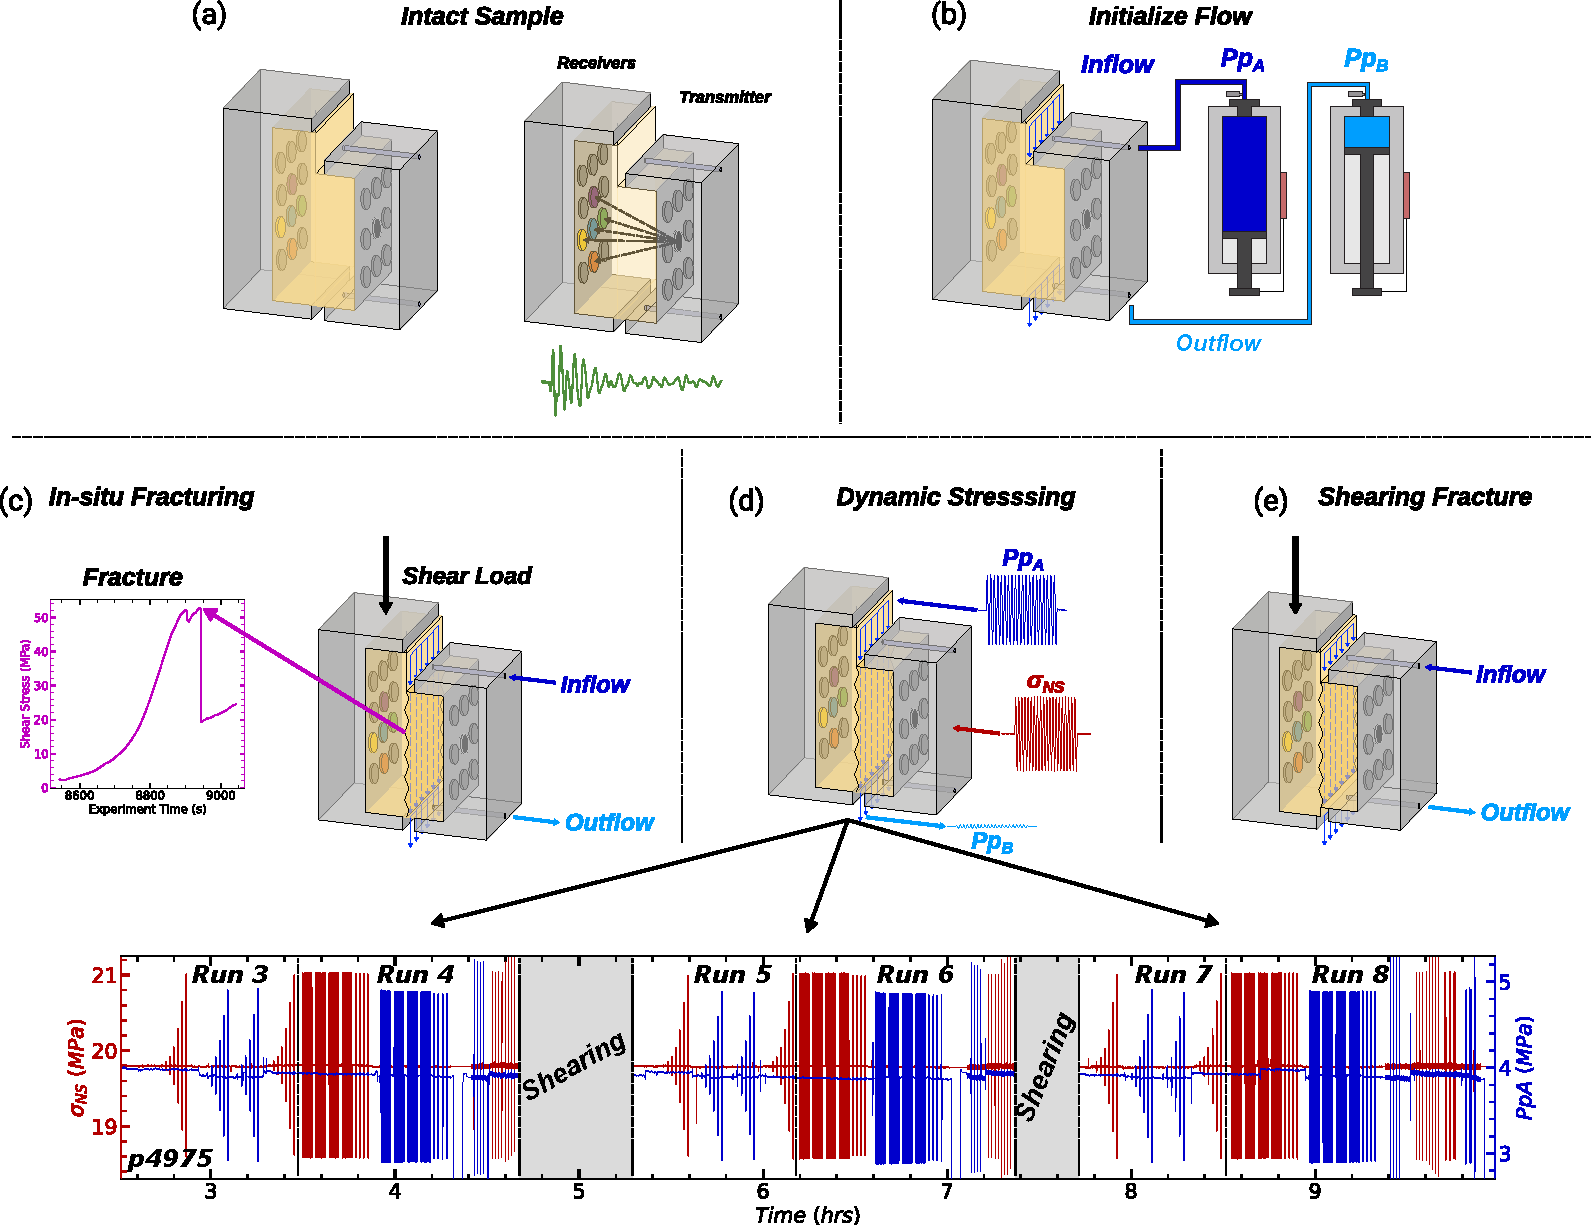
\includegraphics[width=0.99\columnwidth]{exp_sequence_v2}
%	\caption[]{(a) Intact Westerly granite sample cartoon, showing dimensions and approximate transmitter - receiver ray paths. 
%	(b) Next, we applied a pore pressure differential: inlet ($P_{PA}$ = 4 MPa) and outlet ($P_{PB}$ = 2 MPa). 
%	(c) The shear stress was loaded at a constant rate of 10 $\mu m/s$ until reaching the critical shear stress at $ \approx $60 MPa. 
%	(d) Cartoon showing the oscillation protocol applied to the freshly fractured sample. Multiple sets of $P_{P}$ and $ \sigma_{NS} $ oscillations of varying amplitude (up to about $ \pm $ 1 MPa) and frequency (0.1, 1, 10 and 40 Hz) were applied. 
%	(e) The sample was sheared in two additional increments of 4mm, each followed by the dynamic stressing protocol.}
%	\label{fig:exp_seq}
%\end{figure*}
%
%
%\newpage


\section{Results}
\paragraph{}
As previously specified, the ultrasonic waveforms are combined with strain measurements to calculate the nonlinear elastodynamic response and flow rates are used to determine fracture permeability. These measurements allow us to ascertain how the in-situ fracture responds to dynamic stressing. in other words, the imposed oscillations that range in amplitude and frequency probe the elastodynamic and hydraulic properties of the fractured samples. Subsequent results derive from two separate experiments. 

\subsection{Nonlinear elastodynamic and hydraulic responses}
\paragraph{}
Generally speaking, linearly elastic media (of which rocks are not) wave propagation is stress-invariant. Undamaged, unperturbed, rocks do exhibit a modicum of nonlinearity due to microcracks in their matrices and soft grain boundaries (Rivière et al., 2015). When fractured or damaged, rock nonlinear elasticity is furthermore affected by contact acoustic nonlinearity (CAN) at these rough interfaces. The characteristic responses to dynamic stressing (transient softening, velocity modulation, and slow recovery) as shown in Figure \ref{fig:delc_delk_calc}, are indicative of nonlinear mesoscopic elasticity (Guyer and Johnson, 2009) and highly informative on rock microstructure, fractures, and contact mechanics.

\paragraph{}
Through our active source ultrasonic monitoring we characterize the elastodynamic properties of the fractured Westerly granite by quantifying its response to dynamic stressing. Figure \ref{fig:delc_delk_calc} demonstrates typical elastodynamic and hydraulic changes in response to a 1 Hz, 1 MPa normal stress oscillation in experiment number p4966. We characterize the elastodynamic response with three parameters to describe the nonlinearity, $ \Delta c/c_0 $, $ dc/c_0 $, and $ \Delta A/A_0 $. We observe steady-state wave velocity $ c_0 $ before imposed oscillations and are immediately followed by a transient decrease, which eventually heals to a new steady-state wave velocity. That is to say, the fractured rock stiffness of decreases in response to dynamic stressing, quantified by the parameter $ \Delta c/c_0 $. 
The received signal RMS Amplitude, a proxy for energy propagation, evolves in a similar manner as wave velocity, whereby imposed oscillations result in a decrease from the steady-state  $ A_0 $ to a new temporary state. $ \Delta c/c_0 $ and $ \Delta A/A_0 $ quantities demonstrate the transient effect on fracture nonlinearity under dynamic loading conditions, for a range of stress amplitudes and frequencies. 
Another nonlinearity parameter that we identify is modulation in the wave velocity, $ dc $, during oscillations at frequencies that are harmonics of the driving frequency. This represents the average amplitude of these modulations of the wave velocity during dynamic perturbations. Finally, after the stressing the fractured rock exhibits long-term slow dynamics ``recovery'' to the initial $ c_0 $ value, in which the wave velocity evolves to a new, non-equilibrium, steady-state. The rate of wave velocity evolution from post-oscillation to initial $ c_0 $ is fitted with a logarithmic function of the form $ \dot c = p_1\ \log{t} + p_2 $, where $p_1$ is the slope (recovery rate) and $p_2$ is the intercept.

\paragraph{}
Another way to quantify how fractured rock interfaces evolve with dynamic stresses is measuring permeability. In the case of using measuring elasticity, ultrasonic waves propagate orthogonal to the fracture plane and their magnitude and time-delay change depending on how the fracture interface matedness. Hydraulic measurements, comparing inlet and outlet fluid flow across the fracture plane, tell a reciprocal story; permeability and transmissivity reveal how a fracture interface, the porosity, changes. 
The stress-induced changes in permeability are captured by two parameters: (1) The transient change in permeability $ \Delta k/k_0 $ defined as the \%-change due to the imposed normal stress or pore pressure oscillations, normalized by the pre-oscillation permeability $ k_0 $ as illustrated in Figure \ref{fig:delc_delk_calc}c (Candela et al., 2014) and (2) the recovery rate of permeability after the transient increase $ \dot k $. 
Figure \ref{fig:delc_delk_calc} shows the pre-oscillation permeability $ k_0 $ and the post-oscillation permeability $ k = k_0 + \Delta k $ are calculated by averaging the measured values over 10- and 1-s time windows. Calculation discontinuities in permeability measurements shown in Figure \ref{fig:perm_calc} correspond to the data points for which inlet/outlet flow rate difference exceeds the 5\% threshold. Permeability during dynamic stressing is indeterminate because there is no steady-state flow and the diffusion time across the fracture is slower than the higher oscillation frequencies (10 -- 40 Hz). The recovery rate of fracture permeability is quantified by fitting a logarithmic function to the post-oscillation permeability data over a window of 60s. The data is fit to the equation $ \dot k = q_1\ \log{t} + q_2 $, where $q_1$ is the slope (recovery rate) and $q_2$ is the intercept. 

\paragraph{}
To more fully illustrate how the elastodynamic and hydraulic properties of fractured rock change in response to dynamic perturbation we show an excerpt from the post-fracture stage of experiment p4975 in Figure \ref{fig:NS_p4975_run3b_01Hz}. 
Figure  \ref{fig:NS_p4975_run3b_01Hz} demonstrates how the inlet and outlet flow rates evolve during a 0.1 Hz Normal stress oscillation; three colorbars highlight zoomed cycles in the subsequent Figure \ref{fig:bowties}.  During this particular oscillation, there is expected compression and tension in the Normal displacement with increased and decreased Normal stress. The inlet $ Q_A $ flow rate is in phase with the imposed oscillation, but the outlet flow $ Q_B $ is 180$\degree$ out of phase and a much smaller magnitude than that of the inlet;  furthermore, the amplitude trends are modulated throughout the oscillation. The RMS Amplitude and Velocity, as previously discussed, follow the same trend as the Normal stress oscillation, have a modulating amplitude trend, and finally evolve to smaller magnitudes as compared to the commencement of dynamic stressing. 
The relationship between these parameters at the beginning, middle, and end of the oscillation are presented in Figure \ref{fig:bowties}. These hysteresis plots also show how the wave velocity vary as a function of stress. Throughout this long oscillation the velocity-flow hysteresis loop generally evolves to a lower velocity and lower flow rate and the loop becomes more closed. We also observe this general decrease in wave velocity as a function of applied stress throughout the history of the oscillation. These observations demonstrate the magnitude of changes we are characterizing and also reinforce that the fracture is continuously evolving during the dynamic perturbations; contacts undergo compression and tension resulting in changing flow paths across the fracture. 

\paragraph{}
In subsequent subsections we discuss how nonlinear elastodynamic and hydraulic parameters $\Delta c/c_0$, $ \Delta k/k_0 $, $dc/c_0$, and $\Delta A/A_0$ vary with normal stress and pore pressure oscillation amplitudes and frequencies. We also discuss how these results are affected by shearing for both experiments p4966 and p4975. 


%\paragraph{}
%In order to quantify the nonlinearity of the fractures, we first obtain the evolution of ultrasonic wave amplitude (Figure 2b) and velocity (Figure 2c) from the continuously measured ultrasonic data  (Shokouhi et al., 2019) and calculate three parameters: (1) the average or DC-change in wave velocity due to the imposed oscillations, (2) the amplitude of steady-state velocity fluctuation during the oscillations, and (3) the recovery rate of wave velocity post oscillation (Figure 2c). The relative velocity change ($\Delta c/c_0$)
%is defined as the \% change in velocity due to the imposed normal stress or pore pressure oscillation. We calculate $\Delta c/c_0$ 
%from the velocity before ($c_0$) and after ($c$) each oscillation averaged over 1-s time windows as depicted in Figure 2c. At a given oscillation amplitude, the more negative the $\Delta c/c_0$ (larger absolute value), the more nonlinear is the fracture. The parameter 
%$dc/c_0$ is defined as the amplitude of velocity oscillations, averaged over the oscillation duration and normalized by pre-oscillation velocity $c_0$ (Figure X). Similar to $\Delta c/c_0$, a larger magnitude of $dc/c_0$ at a given oscillation amplitude is an indication of higher nonlinearity. The third parameter 
%$\dot c$.
%is defined as the (logarithmic) rate of recovery of wave velocity after the oscillation is removed (Figure 2c). Materials of higher nonlinearity are expected to have slower recoveries (Shokouhi et al., 2017b). In the next section, we discuss the dependence of 
%$\Delta c/c_0$, $dc/c_0$, and $\dot c$ 
%(Figure X) on the imposed normal stress and pore pressure amplitudes as well as frequency.  In addition, we compare the measured nonlinearities before and after shearing the fracture. This comparison provides insight into how changes in the aperture size distribution (due to shearing and wear) and the presence of fines alter the fracture stiffness and the stress-dependency of the elastodynamic response. Although not shown here, similar nonlinearity parameters may be extracted from the evolution of ultrasonic wave amplitude (Figure X). 

%\newpage
%\paragraph{}
%The 90-second hold time between successive oscillations is sufficient for most of the relaxation to take place, although a full recovery may take significantly longer (Renaud, Le Bas and Johnson, 2012). Regardless of the state, the wave velocity follows a time-logarithmic trend as illustrated in Figure 8 for a 1 MPa-oscillation at 10 Hz. This observation is consistent with previous observations (Ten Cate and Shankland, 1996; Shokouhi, Riviere, Guyer, et al., 2017; Shokouhi, Riviere, Lake, et al., 2017), where a late-time time-logarithmic recovery is reported.  
%In order to quantify the recovery rate, the late-time recovery of wave velocity is described by an equation of the form $ c = p_1\ \log{t} + p_2 $, where $p_1$ and $p_2$ are the slope (recovery rate) and intercept respectively. Figure 9 shows the amplitude- and frequency-dependency of the slope $p_1$. We observe that $p_1$ increases with the normal stress oscillation amplitude and decreases with the frequency of oscillations. Of the three-sample states, $p_1$ is the largest for the dry intact sample and smallest for the saturated fractured condition. This observation is consistent with that reported for the other two nonlinearity parameters discussed above. 

\newpage

\begin{figure*}[ht]
	\centering
	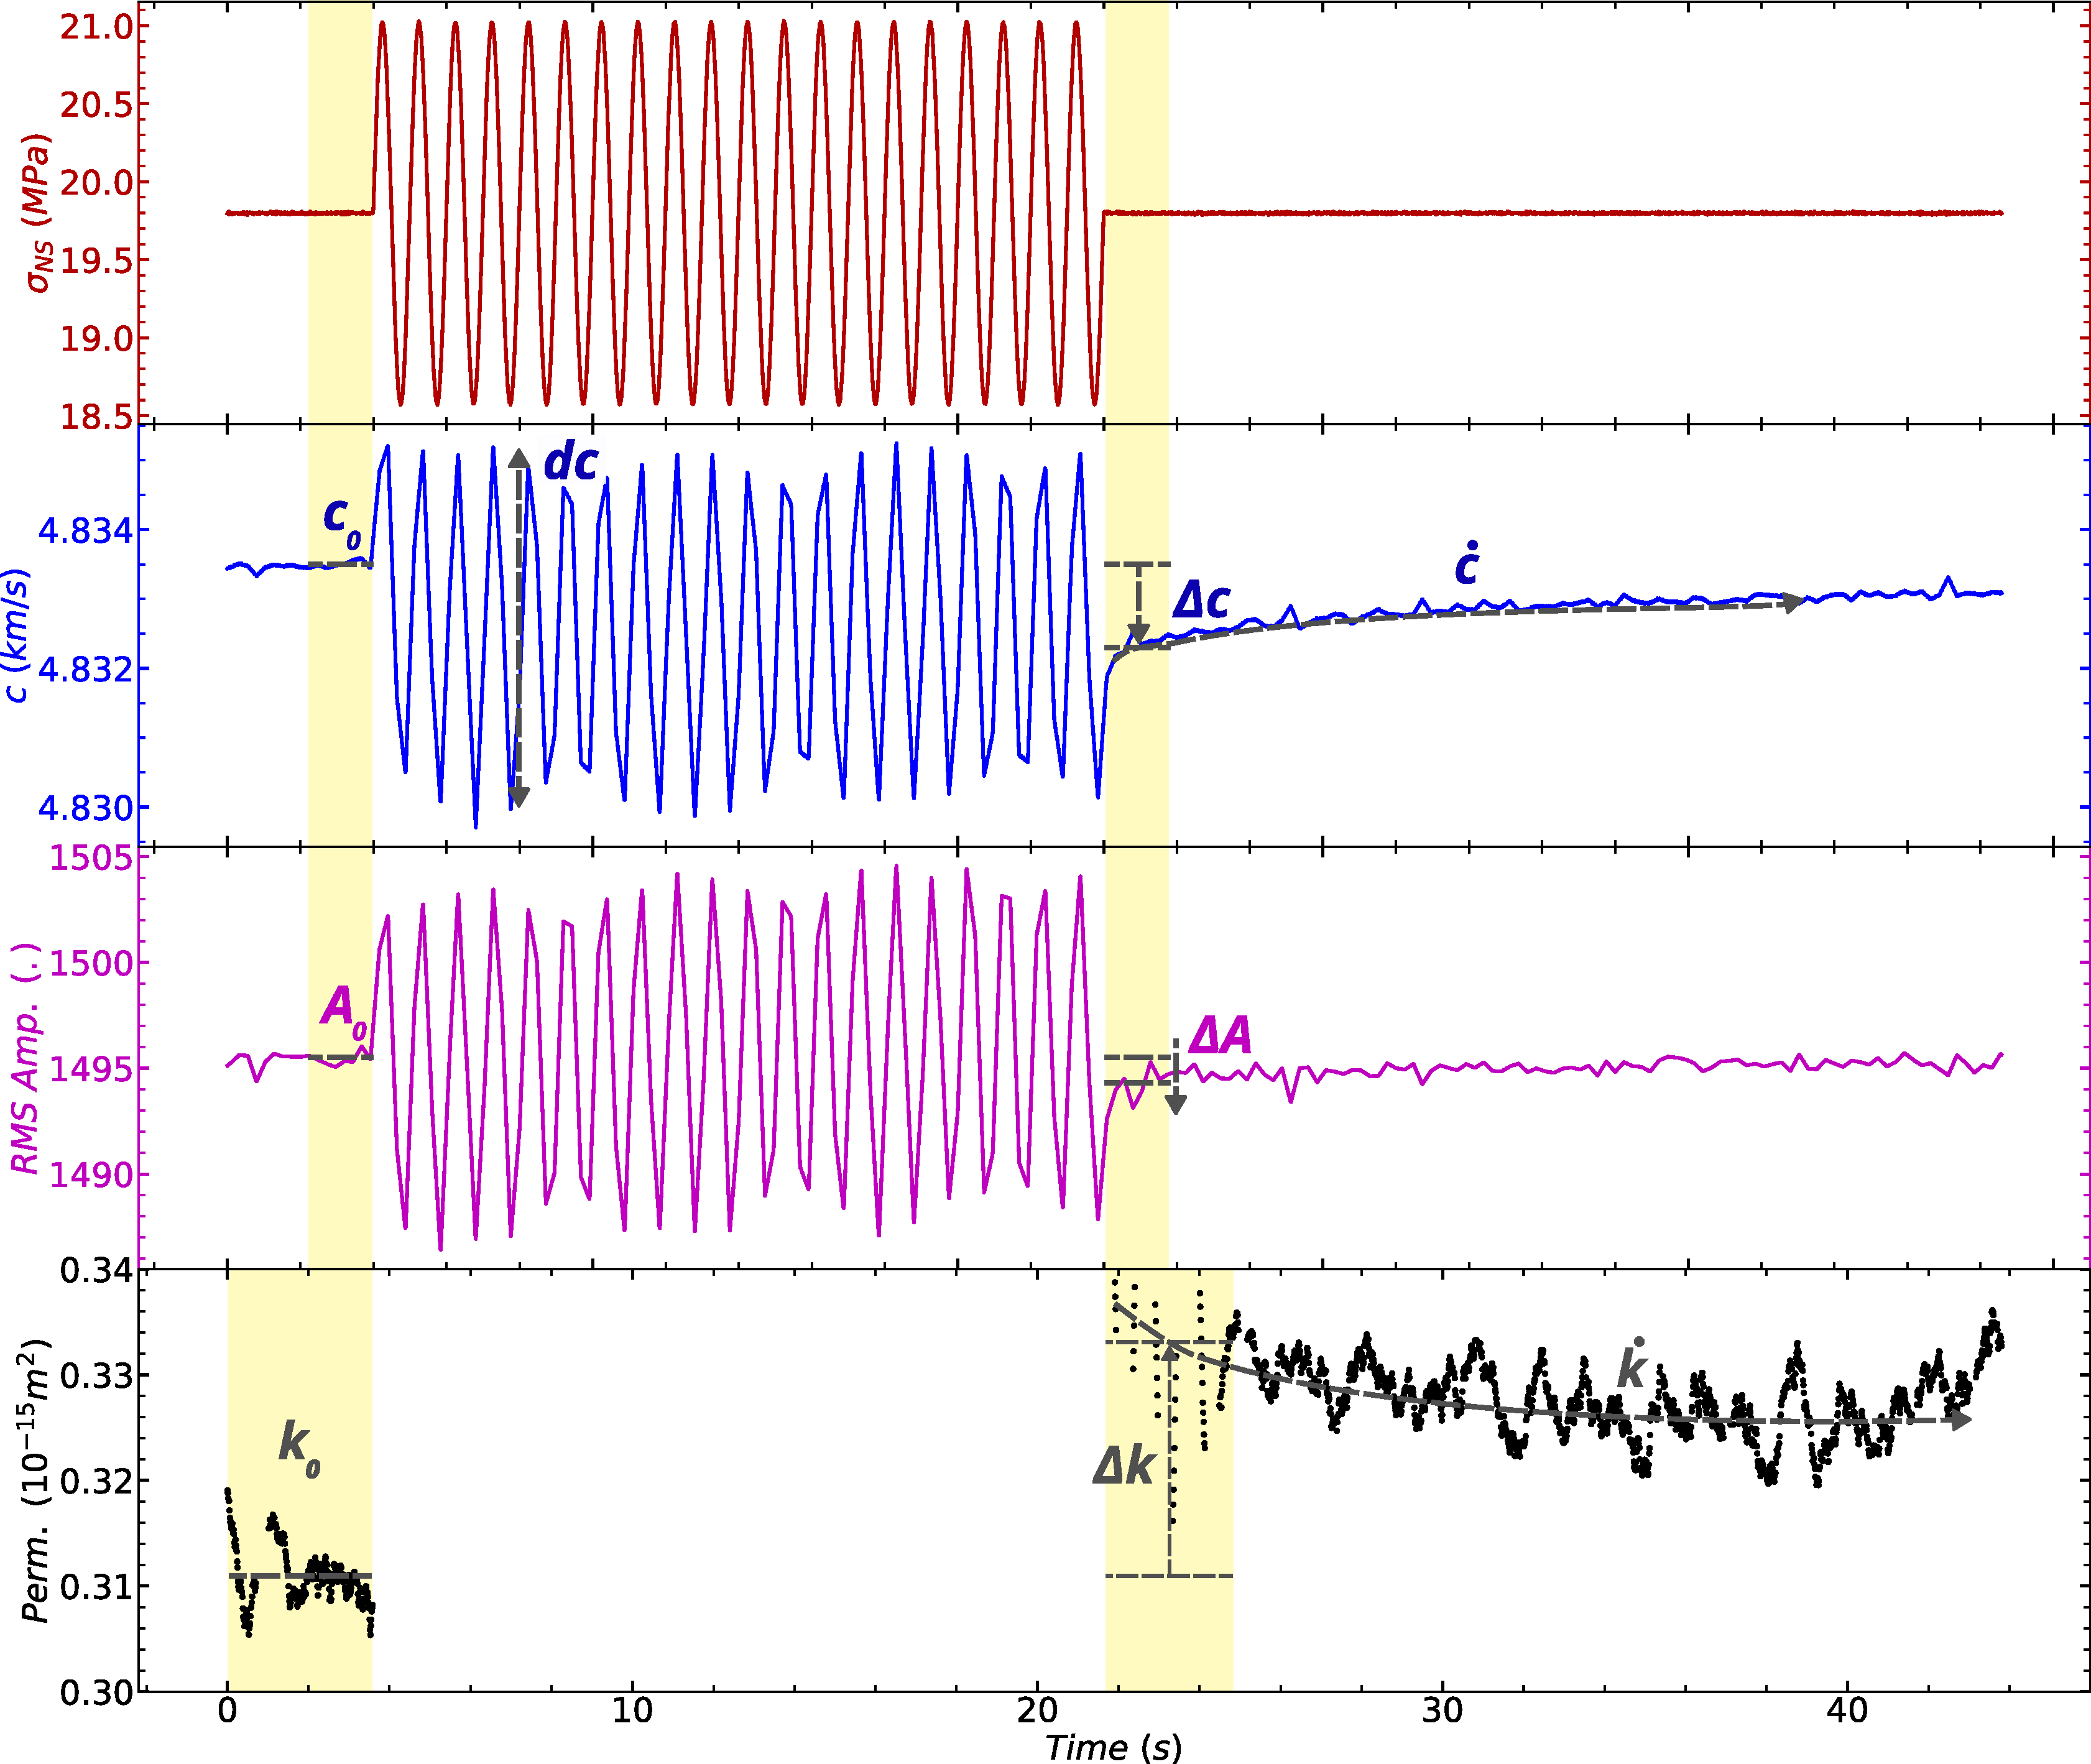
\includegraphics[width=0.9\columnwidth]{NsVelRmsPerm_edit}
	\caption[]{The velocity and permeability changes are calculated using the measured values before and after each oscillation averaged over the time windows (gray boxes) shown in (c). Data points in the permeability measurements are omitted on the condition that inlet/outlet flow rates differ $ > 5 \% $. That is to say, plotted permeability points represent when there is steady-state flow, necessary for Darcy’s law. Dashed lines indicate the recovery of p-wave velocity ($ \dot c$) and permeability ($\dot k$), respectively, from post-oscillation response to new steady-state value. Furthermore, we parameterize the p-wave velocity change $ dc $ during the normal stress or pore pressure oscillations, indicated by dashed blue line.}
	\label{fig:delc_delk_calc}
\end{figure*}

\newpage

\begin{figure*}[ht]
	\centering
	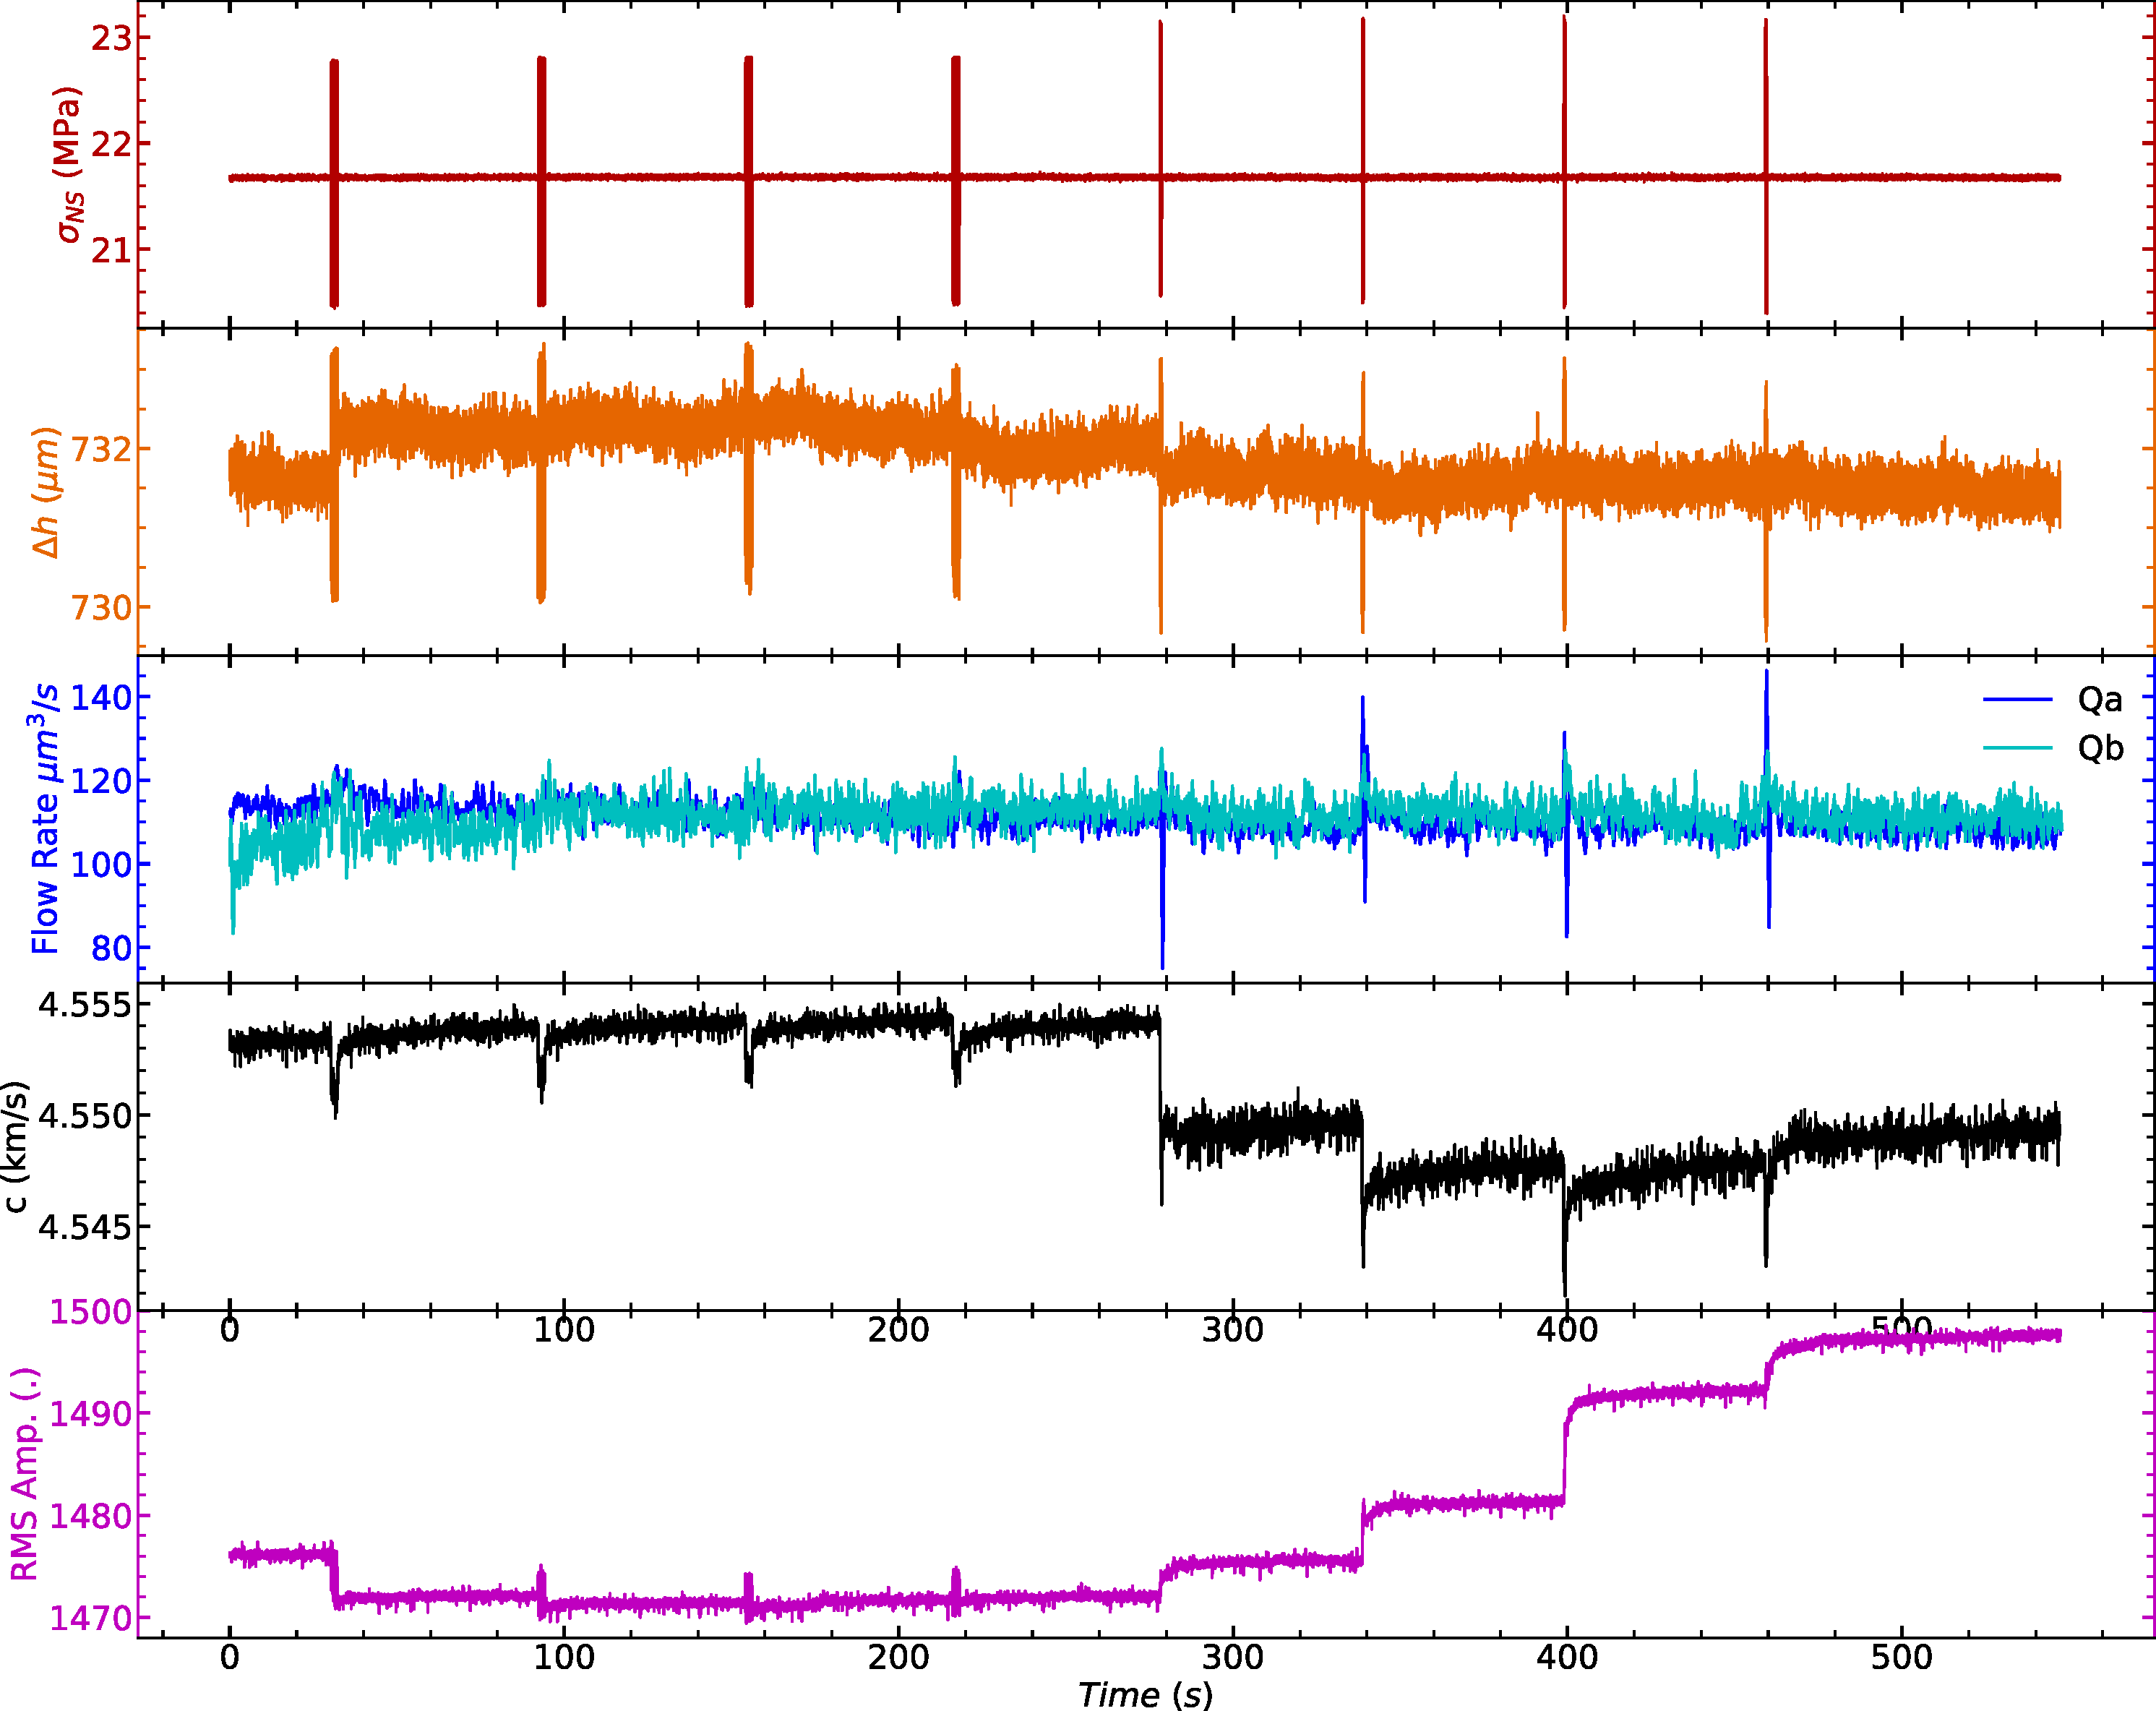
\includegraphics[width=1\columnwidth]{NS_p4975_run4}
	\caption{Run 4 of experiment p4975.}
	\label{fig:run4_p4975}
\end{figure*}

\newpage


%\paragraph{}
%The details on amplitude- and frequency-dependencies of 
%delc/c0 and dc/c0 for a single transmitter-receiver pair are given in Shokouhi et al. (2019). Similar trends are observed for all transmitter-receiver pairs and therefore, not repeated here. In summary, the results given in Shokouhi et al. (2019) indicate that delc/c0 and dc/c0 are modulated by dynamic stress amplitudes for both pore pressure oscillations and fracture normal stress oscillations (Figure 3 and Figure 4). In addition, the measurements exhibit frequency-dependence (not shown here); delc/c0 increases with the oscillation frequency, while dc/c0 mostly decreases. Observing different trends for the different nonlinearity parameters is not surprising. Although the origins of delc/c0 and dc/c0 remain unclear, there is empirical evidence that they stem from different micro-mechanical mechanisms (Riviere et al., 2016, 2015). 
%Although the values tend to generally increase with the oscillation amplitude, we do not observe a clear trend (not shown). This could be in part due to the variability in caused by the low signal-to-noise ratio. The recovery rate does not show a systematic dependency on frequency (not shown).  

%Shearing of the fracture reduces dc/c0 during normal stress oscillations (Figure 4a). Interestingly, we have recorded different post-shear behavior for normal stress vs. pore pressure oscillations; the shearing increases the nonlinearity during pore pressure oscillations for one sample (p4975), while decreasing it for the other sample (p4966) (Figure 4b). This and other observations indicate possible differences in mechanisms activated during these two modes of dynamic stressing. On the other hand, shearing does not have a significant influence on delc/c0. The second shearing step decreases the measured nonlinearity delc/c0 but only slightly.


\begin{figure*}[ht]
	\centering
	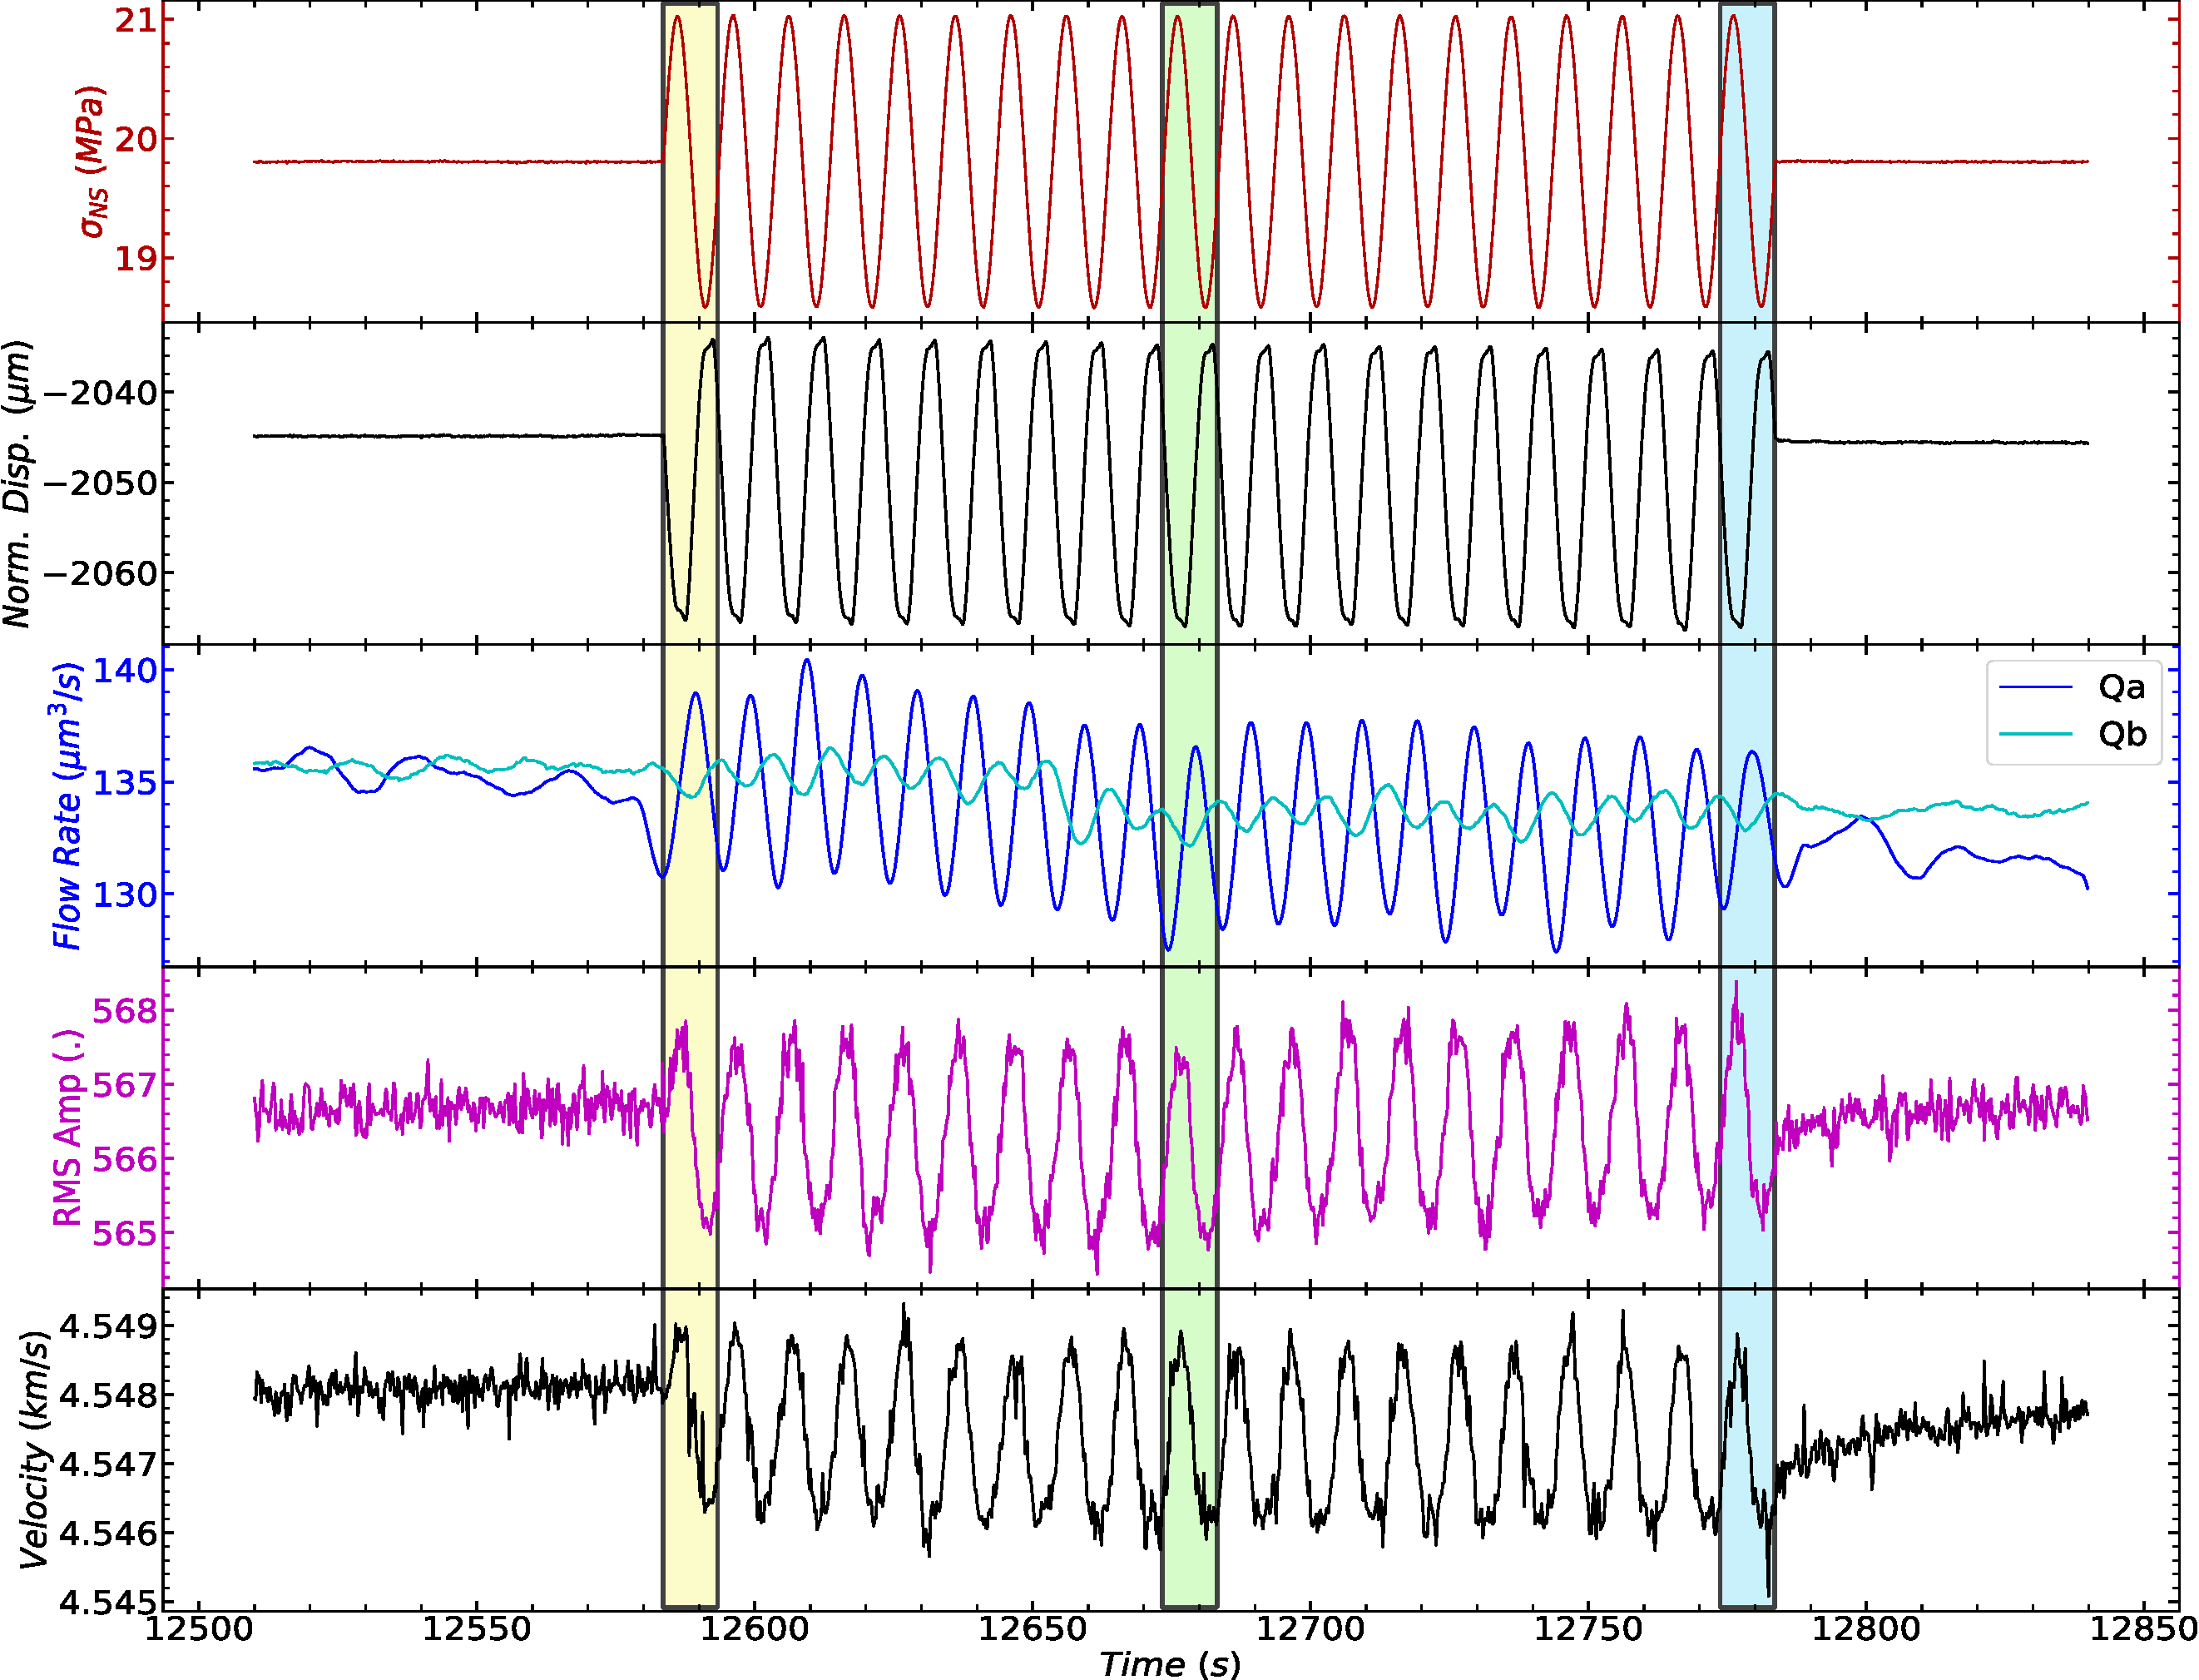
\includegraphics[width=0.8\columnwidth]{plots_bowtie_p4975_run3b_01Hz}
	\caption[]{Direct response of normal displacement, flow rates (inlet and outlet), and ultrasonic RMS amplitude and velocity for the direct path pair during a 0.1Hz 1MPa Normal Stress oscillation. Note the phase delay between the inlet and outlet flow rates. Three sections are highlighted showing one full cycle in the beginning, middle, and end of the normal stress oscillation. }
	\label{fig:NS_p4975_run3b_01Hz}
\end{figure*}


%\begin{figure*}[ht]
\begin{sidewaysfigure}
	\centering
	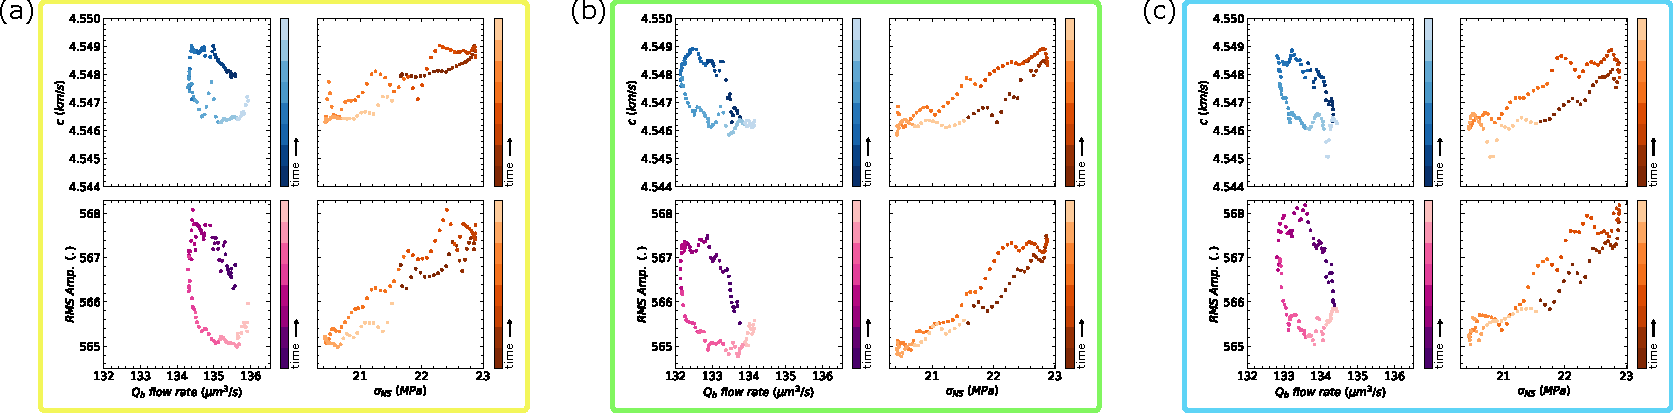
\includegraphics[width=0.9\columnwidth]{bowtie_p4975_run3b_01Hz_v3}
	\caption[]{Evolution of the fracture during a 1 MPa, 1 Hz normal stress oscillation during the first cycle (a), middle cycle (b), and last full cycle (c). The relationship between velocity and RMS Amplitude with outlet flow rate track each other throughout the oscillation, ending in decreased flow. The point to make here is that the fracture is continuously changing -- the change in aperture results in change in velocity and flow paths.}
	\label{fig:bowties}
%\end{figure*}
\end{sidewaysfigure}


\newpage

%\subsection{perm evolution}
%\paragraph{perm evolution: transient response to dynamic stressing \& shear:} 


%\paragraph{Oscillation Amplitude- and Frequency-Dependencies:} 
% Furthermore, for the same oscillation amplitude and frequency, the pore pressure oscillations appear to be more effective in permeability enhancement (delk/k0 $> $ 0) than the normal stress oscillations by a factor of ~2.5, particularly for sample WG1. In addition, delk/k0 increases, albeit slightly, with the frequency of oscillations (not shown here). The only exception is the decrease in delk/k0 for sample WG2, when we increase the fluid pressure oscillations from 1 Hz to 10 Hz. The details on amplitude- and frequency-dependencies of 
%delk/k0 are given in Shokouhi et al. (2019). The recovery rate k. does not show clear amplitude- and frequency-dependencies (not shown here).  
%
%\paragraph{Influence of Shearing:}
%Generally speaking, after shearing the fracture, the normal stress oscillations become less effective in enhancing the fracture permeability (see Figure 5a). The trend is less obvious for pore water pressure oscillations (see Figure 5b). 
%
%\paragraph{correspondence b/w stiffness \& perm transients:}
%The main hypothesis driving this study was that the transient elastic softening is associated with a temporary increase in porosity and/or permeability, both of which are important for energy production and waste storage. Our results to date support this conjecture: the relative changes in wave velocity and permeability of fresh fractures (before shearing), due to both normal stress and pore pressure oscillations, are correlated, such that a larger drop in wave velocity (more negative delc/c0, equivalent to larger transient softening or higher nonlinearity) corresponds to a larger permeability enhancement delk/k0.  As shown in Figures 6a and 6b (left panels), this overall correlaltion seems to hold for both normal stress and pore pressure oscillations. Furthermore, the recovery rates of wave velocity and permeability transients (c. and k.) also seem to be correlated (Figure 7), although there is slightly more scatter. This observation further reinforces the presumed linkage between the evolution of fracture's elastodynamic and flow properties. In other words, the form of the measured permeability transients is similar to that for the nonlinear elastic effects and both recoveries follow the time-logarithmic trajectories observed in the field or in nature. We should note that the correlations shown in Figure 6 correspond to delc/c0 averaged for 5 transducer pairs shown in Figure 1d. Examining the results for individual transducer pairs (not shown here) reveals the strong dependency of the measurements on the wave path. This is not surprising as the fracture aperture is nonuniform and the ray paths sample different portions of that interface. 
%
%Shearing the fracture appears to alter these relations indicating the influence of contact stiffness and shear fabric on both sets of properties (Figure 6a and 6b). Overall, shearing seems to weaken the correlation between delc/c0 and delk/k0 (Figure 6a and 6b, middle and right panels). The question remains as to what underlying micro-mechanisms link the nonlinear elastodynamic behavior and hydraulic properties of fractures. 
%
%We considered two mechanisms for this observed correspondence: (1) the unclogging of fracture flow conduits via fluid pressure oscillations, and (2) the dependence of both properties on stress-induced changes in the fracture aperture. Previous work shows that particle clogging can alter permeability via dynamic stressing in Berea sandstone (Elkhoury et al., 2011; Candela et al., 2014, 2015). However, for fractures in Westerly Granite we observe an increase in permeability for both pore pressure and normal stress oscillations of sufficiently large amplitude. With the new insights from the coupled ultrasonic data, one may conclude that unclogging is merely one of many potential mechanisms. 
%
%The other explanation for the linkage between stiffness and flow properties of fractured rocks could be the dependence of both properties on the fracture aperture change due to the imposed stress oscillations. To further examine this hypothesis, we investigated whether delc/c0 or delk/k0 correlate with the measured changes in sample thickness changes (proxy for aperture compaction/dilation) during imposed oscillations (Shokouhi et al., 2019). However, we did not observe a strong correlation. This lack of strong correlation suggests that changes in fracture aperture cannot be the sole driving mechanism for permeability change, especially when driven by pore pressure oscillations.                          

%\paragraph{From Prabaha's Arma:}
%The nonlinear parameter delc/c0 is plotted against the applied normal stress oscillation amplitude (0.2-1MPa) in Figure 5. The sample is more nonlinear if the absolute value of 
%delc/c0 is larger at a given oscillation amplitude and frequency. As shown in Figure 5 (a) 
%delc/c0 of the intact sample increases as the normal stress amplitude increases. Also, the nonlinearity seems to increase with the oscillation frequency. This trend closely resembles previous observations in dry intact Berea sandstone (Riviere et al., 2016). Similar trends are observed for the fractured sample in dry (Figure 5 (b)) and saturated (Figure 5 (c)) states. The results for the saturated fractured sample at 1Hz are also comparable to our previous observations on in-situ-stressed fractured samples of Westerly granite (Shokouhi et al., 2019).  
%\paragraph{}
%Figure 7 shows the normal stress amplitude- and frequency-dependency of the second extracted nonlinearity parameter dc/c0 for the sample in the three states. Similar to delc/c0, dc/c0
%scales linearly with amplitude although, the trend here is clearer. Similar to what was observed for delc/c0, the dry intact sample appears more nonlinear than the dry fractured sample, which exhibits more nonlinearity than the saturated fractured sample.  

%\newpage


\subsection{Nonlinear Elastodynamic Response: Relative Changes in Permeability and Velocity}
\paragraph{}
The hypothesis driving this work and future studies is that transient elastic softening in dynamically stressed fractured rock corollary  increase in porosity and/or permeability. A more complete understanding this is important for both natural phenomena for energy production and waste storage. 
%Our results to date support this conjecture: the relative changes in wave velocity and permeability of fresh fractures (before shearing), due to both normal stress and pore pressure oscillations, are correlated, such that a larger drop in wave velocity (more negative delc/c0, equivalent to larger transient softening or higher nonlinearity) corresponds to a larger permeability enhancement $ \Delta k/k_0 $.  As shown in Figures 6a and 6b (left panels), this overall correlation seems to hold for both normal stress and pore pressure oscillations.The gray dashed lines in these figures at $ k = k_0 + \Delta k $ mark the boundary between permeability increase and decrease due to the imposed oscillation.

The dependency of $ \Delta k/k_0 $ on the amplitude Normal stress and pore pressure oscillations are shown in Figure \ref{fig:perm_ns_amp}, which additionally differentiates the order in which the 1 Hz oscillations sets were imposed. We observe the relative permeability change $ \Delta k/k_0 $ generally scales with the amplitude of 1 Hz Normal stress and pore pressure oscillations and that the order in which oscillations were conducted have an effect on the permeability enhancement. There are cases where small oscillation amplitudes ($< $ 0.5MPa) result in a modest reduction in permeability for Normal stress oscillations, but can result in relatively larger reductions from Pore pressure modulation. Despite scatter, there is similar relationship between the two separate fractures, experiments. 

Order of oscillations does not necessarily correlate to a specific permeability enhancement or reduction, but does have an effect on the overall results. This is most likely due to the fact that the Pore pressure and Normal stress oscillations do not strictly alternate, although the order is consistent in post-fracture, post-shear 1, and post-shear 2 parts of the experiments. 

We observe in experiments p4966 and p4975 similar results in $ \Delta k/k_0 $ for the post-fracture case. This is not entirely surprising because, though these are different in-fractures, they are both Westerly granite and were under the same loading conditions to produce planar fractures with presumably similar apertures and amount of fragmentation. This similarity deteriorates especially with Pore pressure oscillations after the first shear phase of the experiments. After shearing the fractures 5 mm fragmented wear material developed in the interface and thus allows for more complicated flow -- clogging and unclogging during the Pore pressure oscillations where wear material was dislodged from certain parts of the fracture or were lodged in other parts.  

Furthermore, $ \Delta k/k_0 $ is mostly unaffected or is reduced during Normal stress oscillations for post-shear cases. Gouge material generated from shear was not mobilized the degree to which was observed in Pore pressure oscillations because the Pore pressure was not dynamically acting on the gouge material and the Normal stress oscillations may not have opened the fracture enough for movement of gouge material. This mechanism is not fully understood but likely plays a significant role in this complicated process.

\clearpage

\begin{figure*}[ht]
	\centering
	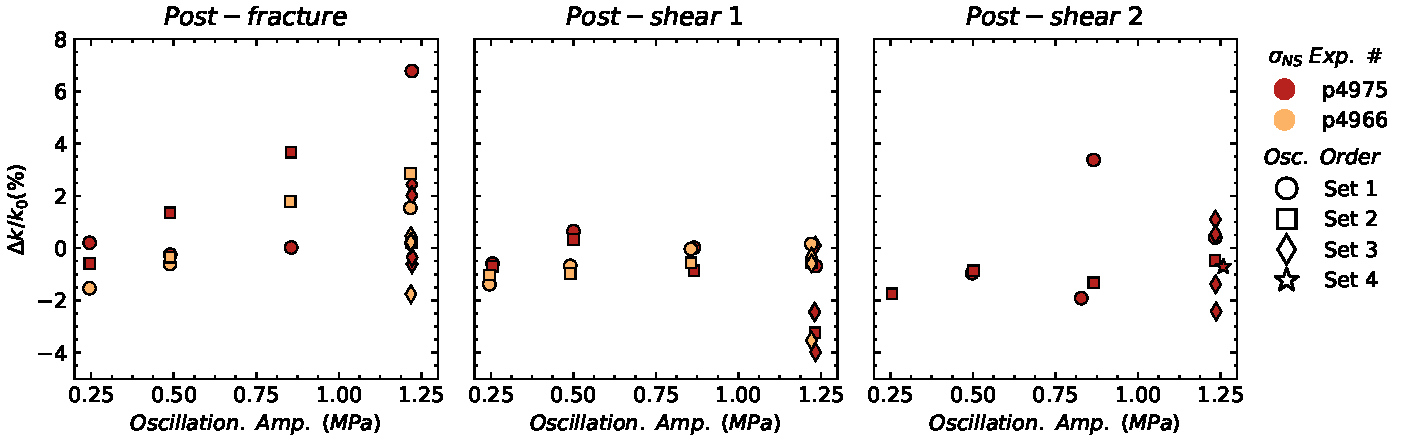
\includegraphics[width=1\columnwidth]{delk_amp_NS}
	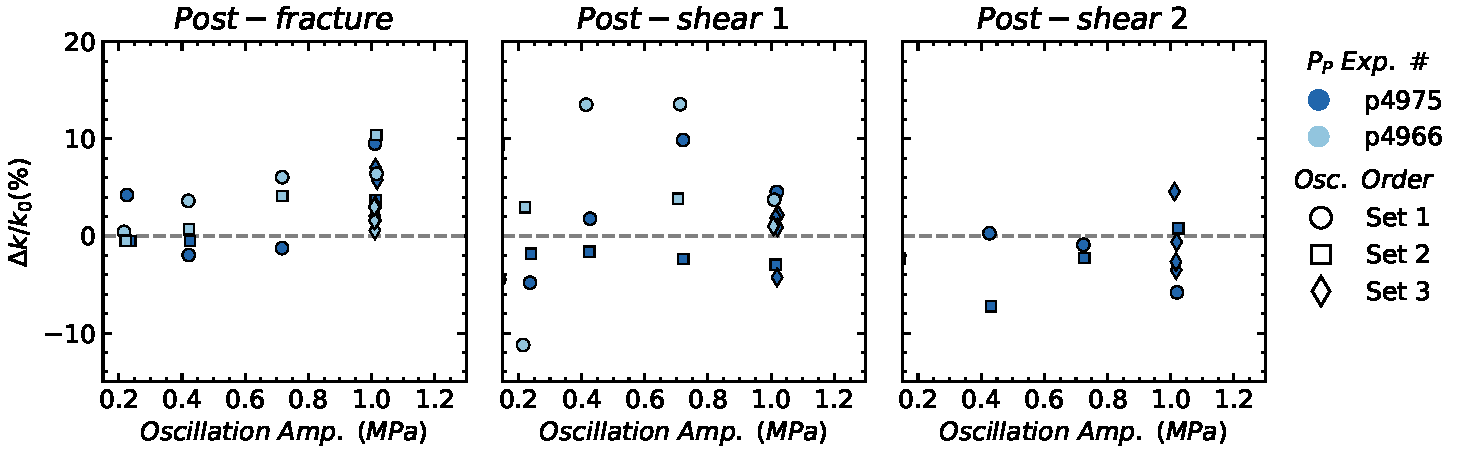
\includegraphics[width=1\columnwidth]{delk_amp_PP}
	%\enspace
	%\includegraphics[width=6cm]{post-frac_amp_array}
	\caption{Relative change in permeability as a function of $ \sigma_{NS} $ and $ P_p $ oscillation amplitude. Transitioning from post-fracture results to post-shear, we observe decreased permeability enhancement. Clogging from in-situ fracture gouge and subsequent gouge development from shear may impede flow through flow paths along the fracture plane.}
	\label{fig:perm_ns_amp}
\end{figure*}

\clearpage

\paragraph{}
For the purpose of explanation, the relative change in velocity $ \Delta c/c_0 $ for the direct transmitter-receiver pair as a function of 1 Hz Normal stress and pore pressure amplitude oscillations are plotted in Figure \ref{fig:delc_ns_amp}. We observe increasing nonlinearity (more negative $ \Delta c/c_0 $) with oscillation amplitude for both Normal stress and pore pressure. This general relationship is similar for Normal stress, but there appear to be two slightly different trends for the respective experiments during Pore pressure oscillations. 

In this measure of fracture nonlinearity there is a clearer trend between oscillation order and magnitude, for this transmitter-receiver path. Normal stress oscillations for the post-fracture case exhibit a more linear elastic fracture subsequent oscillation sets, which is relatively absent from imposed Pore pressure oscillations. 

The effect of shear on fracture nonlinearity is more obvious for Pore pressure oscillations and rather scattered for applied Normal stress oscillation sets. Interestingly the nonlinearity relationship with amplitude barely changes with amount of shear for p4975; though p4966 there is change from the post-fracture case to a greater magnitude of nonlinearity. However, for applied Normal stress successive shear scatters the trend we observe in post-fracture sets, presumably deriving from dramatic changes the fracture surface asperities fracture aperture have undergone through the process of shear displacement. This is investigated further with the analysis of all available transmitter-receiver pairs measurement of nonlinearity. 

\clearpage

\begin{figure*}[ht]
	\centering
	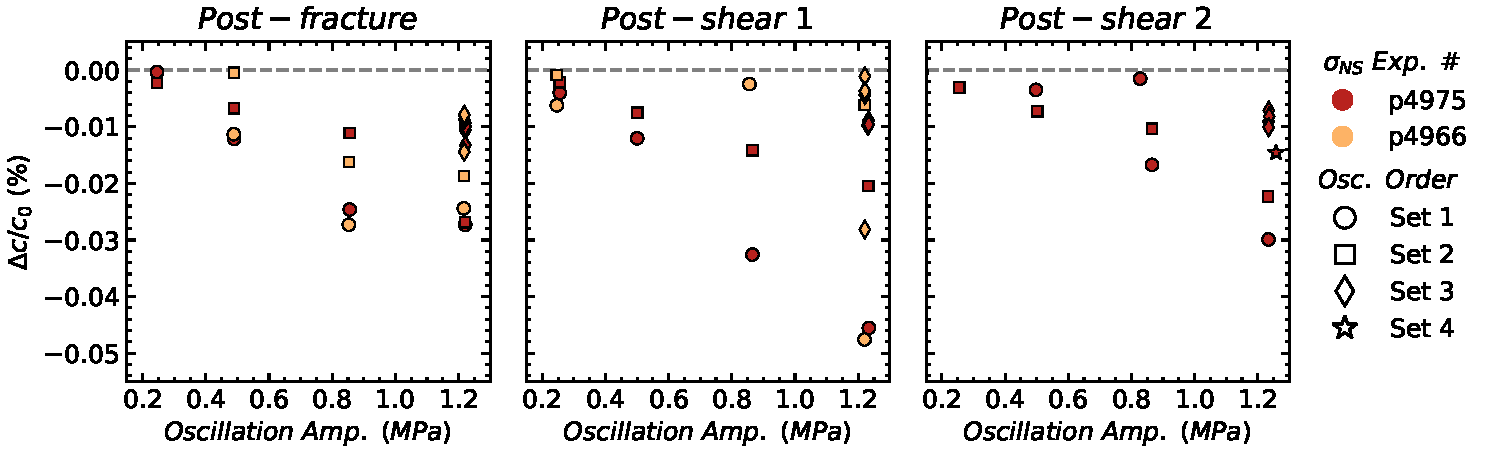
\includegraphics[width=1\columnwidth]{delc_amp_NS}
	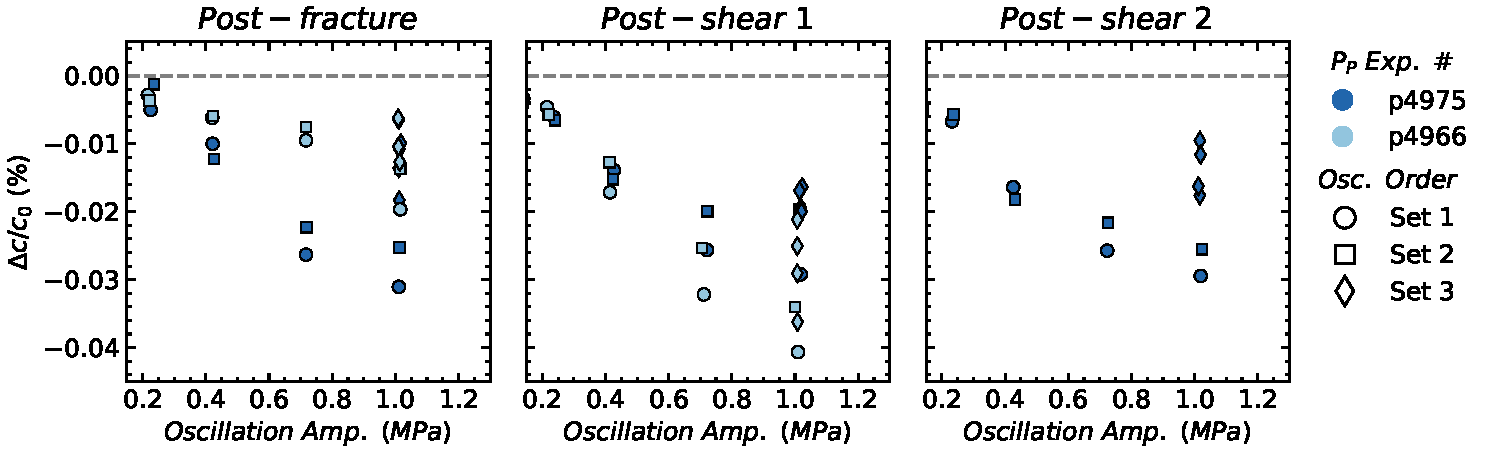
\includegraphics[width=1\columnwidth]{delc_amp_PP}
	%\enspace
	%\includegraphics[width=6cm]{post-frac_amp_array}
	\caption{Nonlinearity as a function of $ \sigma_{NS} $ and $ P_p $ oscillation amplitude. Transitioning from post-fracture results to post-shear results, we observe decreased and more scattered nonlinearity.}%
	\label{fig:delc_ns_amp}
\end{figure*}

\clearpage


%\subsection{Nonlinear Elastodynamic Response: Relative Changes in Permeability and Velocity}
\paragraph{}
We have investigated how fracture nonlinearity changes with successive shear by analyzing all available transmitter-receiver pairs measurement of wave velocity, shown in Figures \ref{fig:delc_plots_ns} -- \ref{fig:delc_plots_pp}. Figure \ref{fig:delc_plots_ns} shows a coarse view of the nonlinear elastodynamic response across the fracture as a function of applied oscillation amplitude; additionally, the data point shapes correspond to oscillation frequencies. The direct path sensor shows a general trend of increasing nonlinearity with Normal stress oscillation and frequency, in both experiments. The other sensors measure more scatter and also more linearity in the case of the bottom sensor of p4975. The effect of shearing reduces nonlinearity (direct pair) and modestly increases nonlinearity (top sensor path), but does not have an overall coherent trend for both experiments and all increments of shear. 
The story for Pore pressure oscillations, Figure \ref{fig:delc_plots_pp}, show more coherent results as compared to Normal stress. Again, there is a general trend in increasing nonlinearity with amplitude and oscillation; it is interesting the bottom receiver path exhibits markedly lower nonlinearity. Furthermore, there is much more similarity in results for the separate experiments than observed in the Normal stress oscillations. Another important observation is that shearing has little effect on the magnitude of nonlinearity for Pore pressure oscillations. 

These scattered results are not expected as the fracture has a heterogeneous aperture and gouge composition, especially with application of shear displacement. It is conceivable that shear increases the aperture in some locations, which could be filled with gouge material or empty, and other parts of the fracture aperture could be closed. These possibilities may be partially responsible for the complicated behavior we observe. 

A way to probe this further is determining the degree to which the between contact stiffness and the hydraulic properties of the fractures during dynamic stressing are interrelated. Figure \ref{fig:delc_plots2} relates permeability changes $ \Delta k/k_0 $, a hydraulic measurement averaged across the fracture plane, to the change in wave velocity $ \Delta c/c_0 $ averaged across all receiver locations. The data point shapes correspond to the oscillation frequencies and their sizes correspond to oscillation amplitude. The main observation for the post-fracture oscillation sets is that relative changes in permeability and wave velocity are correlated. That is to say, larger Normal stress or Pore pressure oscillation amplitude and frequencies produce larger transient softening and permeability enhancement. Overall, shear weakens this relationship, reducing the amount of nonlinearity and permeability enhancement for both methods of dynamic stressing. Though, in the case of Normal stress oscillations, the relationship with amplitude and frequency still exists, just the overall slope decreases due to shear displacement. 

We conjecture that nature of the correspondence between nonlinear elastodynamic and hydraulic properties of fractured rock depend on clogging mechanisms. During both types of dynamic stressing flow conduits across the fracture are clogged/unclogged in a complicated fashion, resulting in mobilization of gouge material (generated from in-situ fracture and subsequent shear displacement) and permeability enhancement/reduction. Though has been in observed in previous studies of Berea sandstone (Elkhoury et al., 2011; Candela et al., 2014, 2015), we observe permeability enhancement in for Normal stress and Pore pressure oscillations (for amplitudes $ > 0.5 $  MPa). Thus, fracture asperity changes from stressing and clogging mechanisms account for a minority of the rich underlying physics.     

%Shearing the fracture appears to alter these relations indicating the influence of contact stiffness and shear fabric on both sets of properties (Figure 6a and 6b). Overall, shearing seems to weaken the correlation between Δ𝑐⁄𝑐5 and Δ𝑘⁄𝑘5(Figure 6a and 6b, middle and right panels). The question remains as to what underlying micro-mechanisms link the nonlinear elastodynamic behavior and hydraulic properties of fractures.
%We considered two mechanisms for this observed correspondence: (1) the unclogging of fracture flow conduits via fluid pressure oscillations, and (2) the dependence of both properties on stress-induced changes in the fracture aperture. Previous work shows that particle clogging can alter permeability via dynamic stressing in Berea sandstone (Elkhoury et al., 2011; Candela et al., 2014, 2015). However, for fractures in Westerly Granite we observe an increase in permeability for both pore pressure and normal stress oscillations of sufficiently large amplitude. With the new insights from the coupled ultrasonic data, one may conclude that unclogging is merely one of many potential mechanisms.
%The other explanation for the linkage between stiffness and flow properties of fractured rocks could be the dependence of both properties on the fracture aperture change due to the imposed stress oscillations. To further examine this hypothesis, we investigated whether Δ𝑐⁄𝑐5 or Δ𝑘⁄𝑘5 correlate with the measured changes in sample thickness changes (proxy for aperture compaction/dilation) during imposed oscillations (Shokouhi et al., 2019). However, we did not observe a strong correlation. This lack of strong correlation suggests that changes in fracture aperture cannot be the sole driving mechanism for permeability change, especially when driven by pore pressure oscillations.
%We also used high-resolution optical profilometry to measure the roughness across the post-mortem fractured surfaces in order to reconstruct the fracture aperture distribution. However, since the fractures were created in- situ and were sheared twice before the roughness measurements, we do not have information on the aperture or roughness of fracture interfaces immediately post-fracture nor immediately post-shear (1st shearing step).

%\subsection{Relative Change in Velocity and Permeability: Ray Paths}

\begin{figure*}[ht]
	\centering
	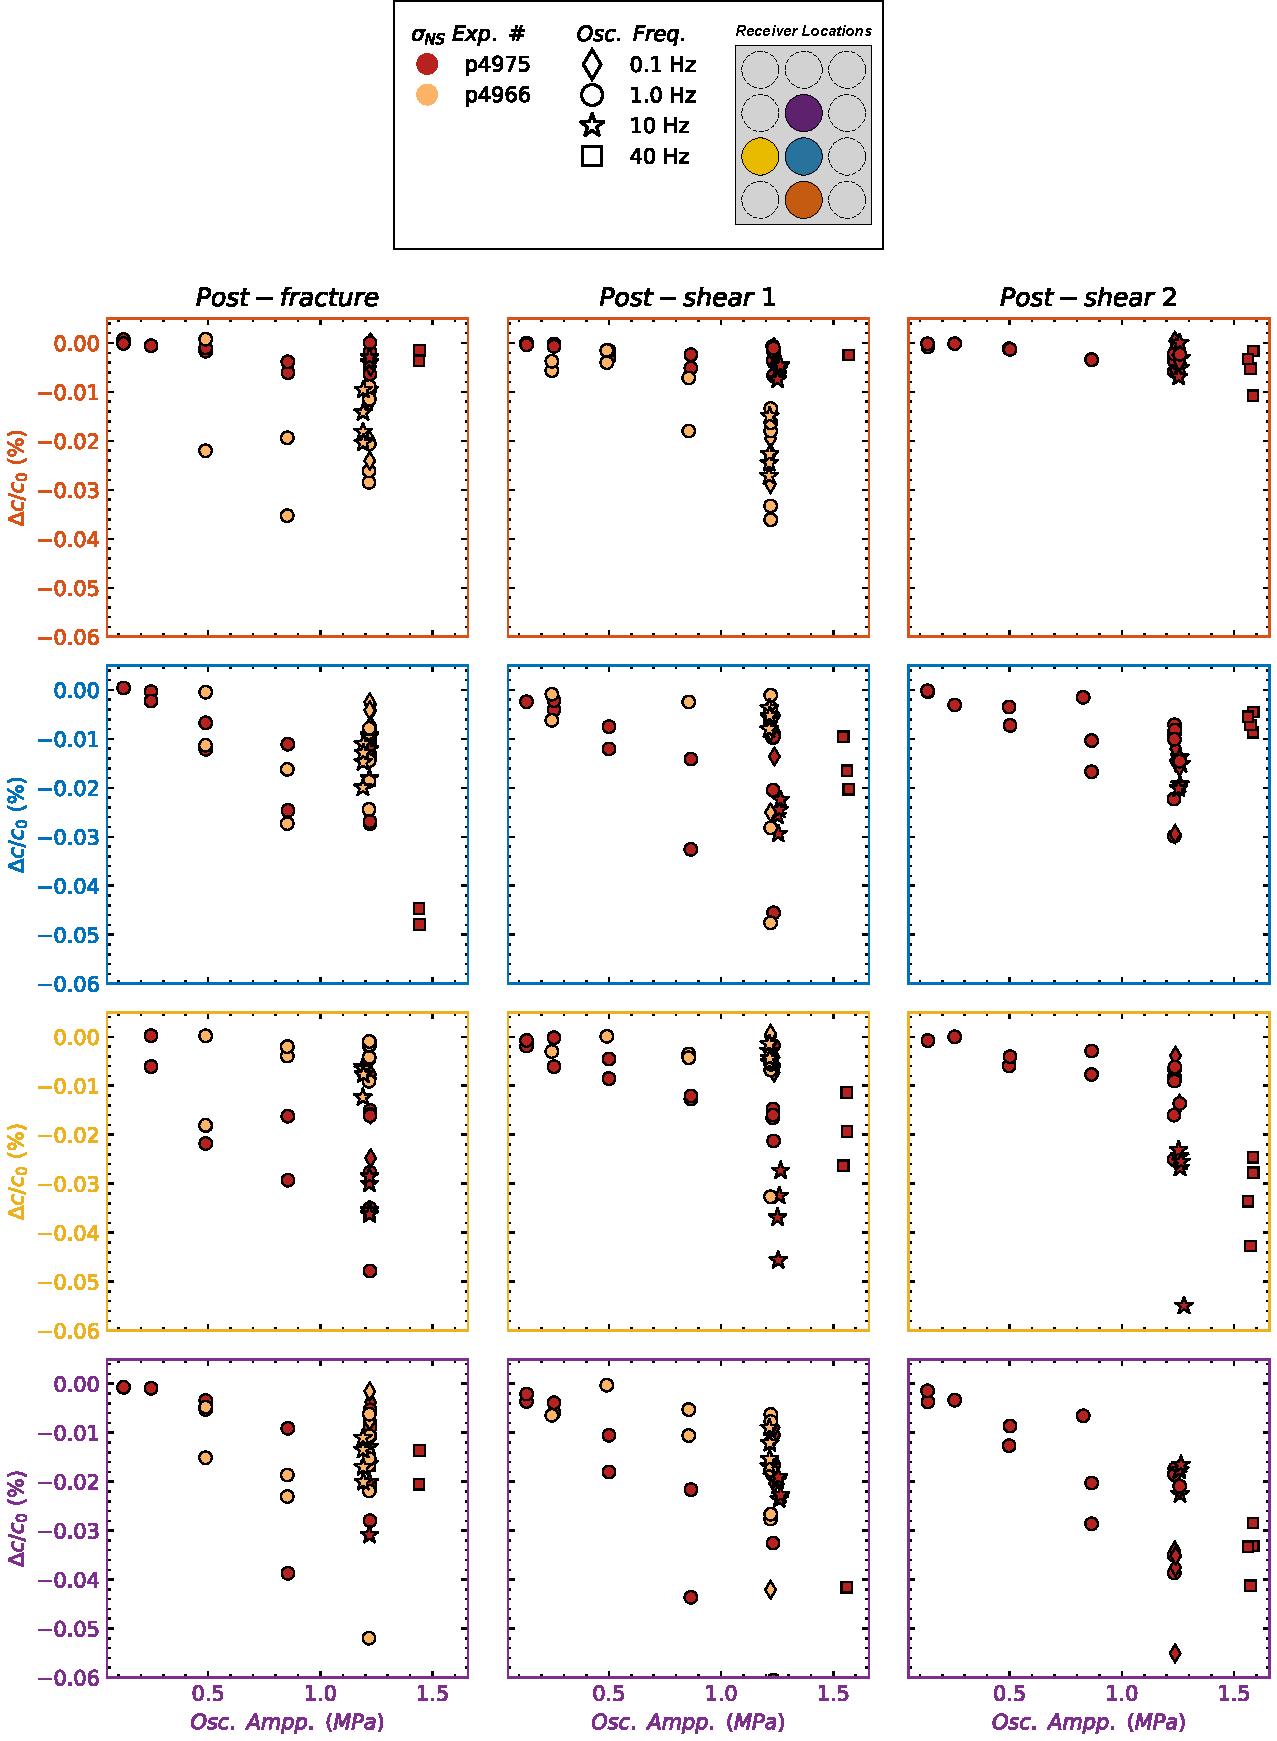
\includegraphics[width=0.9\columnwidth]{Delc_bypair_all_NS}
	\caption{Nonlinearity as a function of $ \sigma_{NS} $ oscillation amplitude for each receiver. Transitioning from post-fracture results to post-shear results, we observe decreased nonlinearity.}
		\label{fig:delc_plots_ns}
\end{figure*}

\clearpage

\begin{figure*}[ht]
	\centering
	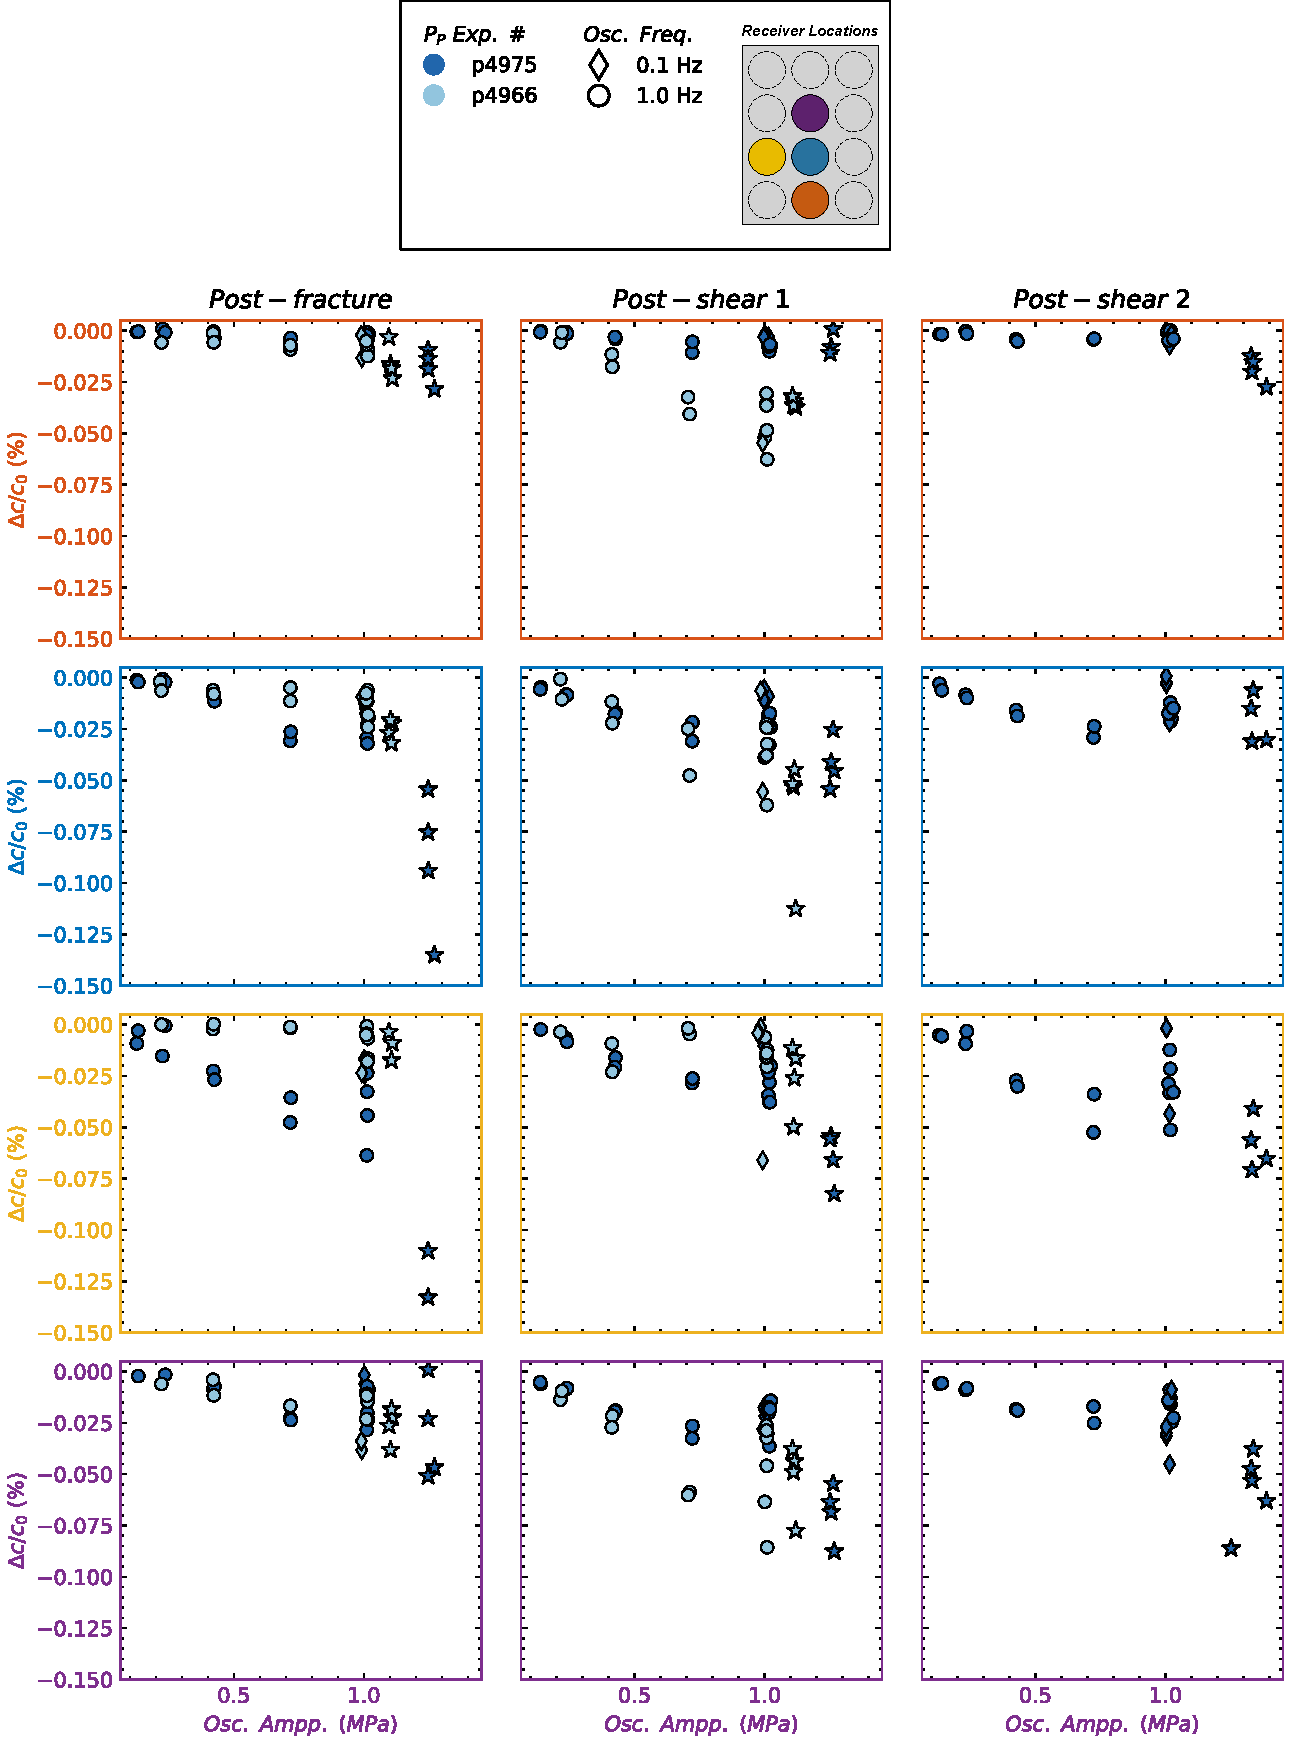
\includegraphics[width=0.9\columnwidth]{Delc_bypair_all_PP}
	\caption{Nonlinearity as a function of Pore pressure oscillation amplitude for each receiver. Transitioning from post-fracture results to post-shear results, we observe decreased nonlinearity.}
		\label{fig:delc_plots_pp}
\end{figure*}

\clearpage


\begin{figure*}[ht]
	\centering
	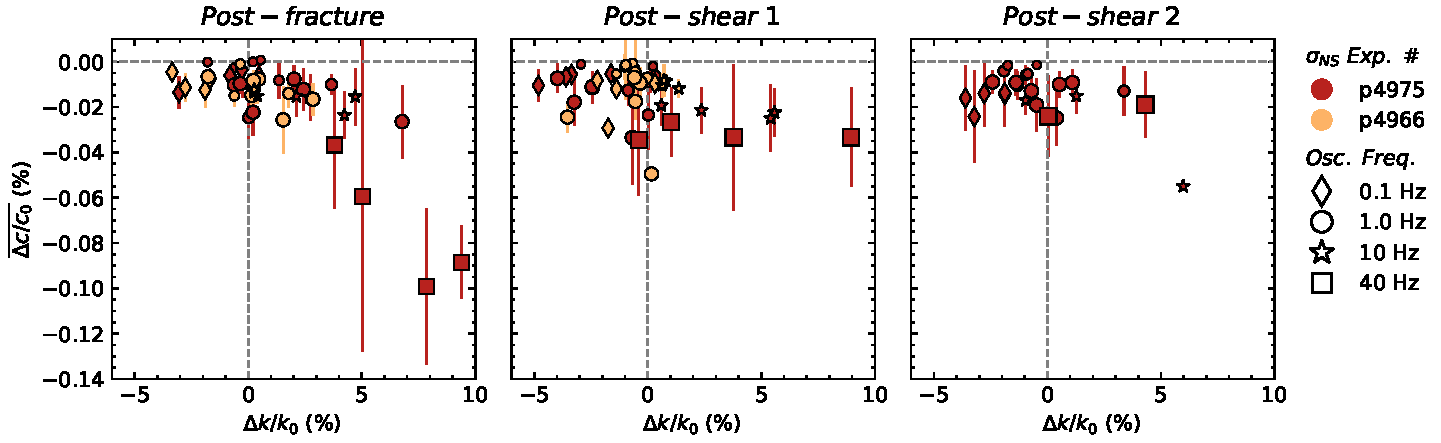
\includegraphics[width=1\columnwidth]{avgDelc_All_ampsNS}
	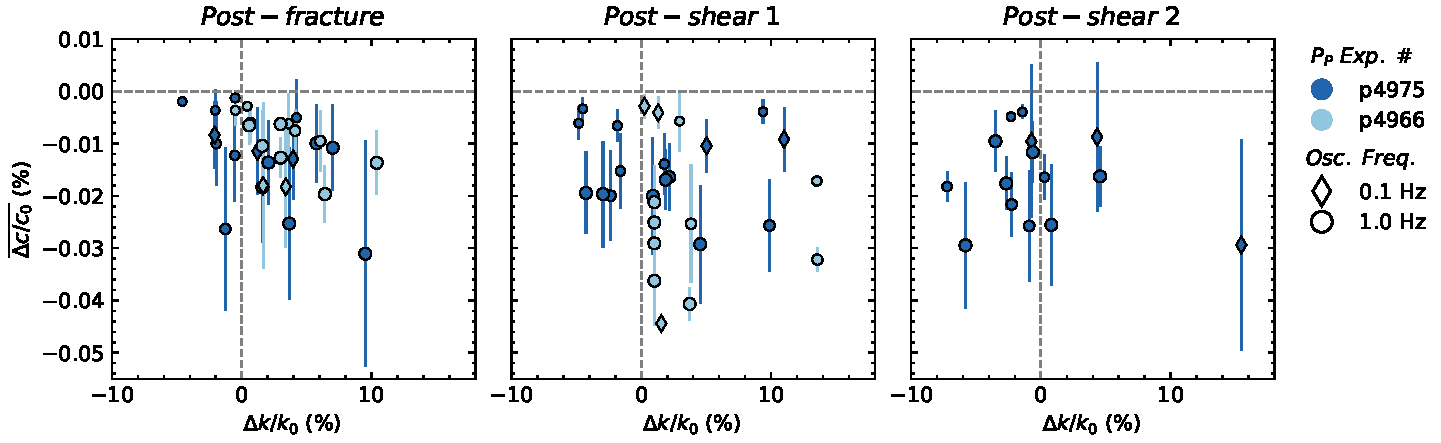
\includegraphics[width=1\columnwidth]{avgDelc_All_ampsPP}
	%\enspace
	%\includegraphics[width=6cm]{post-frac_amp_array}
	\caption{Nonlinearity as a function of permeability change for $ \sigma_{NS} $ and $ P_P $ oscillations averaged over all receivers. Data point shapes correspond to the oscillation frequencies and their sizes to amplitude. In post-fracture oscillation sets relative changes in permeability and wave velocity are correlated. That is to say, larger Normal stress or Pore pressure oscillation amplitude and frequencies produce larger transient softening and permeability enhancement. Overall, shear weakens this relationship, reducing the amount of nonlinearity and permeability enhancement for both methods of dynamic stressing. }
	\label{fig:delc_plots2}
\end{figure*}

\clearpage


\subsection{Nonlinear Elastodynamic Response: Relative Change in RMS Amplitude}
The change in RMS amplitude, $ \Delta A/ A_0 $, more or less evolves in a similar manner with applied oscillation amplitude (see Figure \ref{fig:delA_ns_amp}) as $ \Delta c/c_0 $. In the post-fracture case p4975 results shows that the change in transmitted p-wave amplitude becomes more negative with increasing Normal stress excitation amplitude; this trend is minor with Pore pressure oscillation amplitude. Furthermore, there is little variation in these results with order of which the oscillations were conducted. The situation is different for experiments p4966 in that the results are very scattered for Normal stress oscillations and more coherent for Pore pressure oscillations. The order of oscillation is most pronounced for oscillation amplitudes $ > 0.25 $ MPa, subsequent sets are less nonlinear. Surprisingly, Normal stress oscillations in post-shear 1 of experiment p4966 produce positive changes in RMS amplitude, which contradict our findings with respect to $ \Delta c/c_0 $. Another interesting observation is that progressive shearing creates conditions that produce less nonlinearity. 

The averaged change in RMS as a function of $ \Delta k/k_0 $ is plotted in Figure \ref{fig:dela_plots2}. These plots show a complex relationship between the transmitted spectral energy and fracture hydraulic properties. Normal stress oscillations of 40 Hz frequency consistently produce positive nonlinearity values. This and our observation that nonlinearity decreases with shearing are in fact physical rather than artifacts of data analysis, detailed in Supplemental Section X. Pore pressure oscillation results are more scattered but show a similar relationship as Normal stress oscillations, but the underlying elasto-hydraulic mechanisms require further experimental investigation.  

%\textit{\textcolor{red}{Attached are two papers from Tutuncu, and Claytor/TenCate (fig. 1) regarding frequency/strain rate dependencies. \\
%From quasi-static tests, when the sample is driven slowly, all the contacts have enough time to ‘recover’ from the disturbance, leading to little/no hysteresis. \\
%This is consistent with DAET experiments (intact Berea sample), where we also see an general increase in softening (larger increase in $ \delta c/c_0 $) with frequency. Contacts don’t have enough time to age back to their original states when the oscillation frequency is high.}}


%\begin{itemize}
%	\item Although the origins of $dc/c_0 $ and $ dc/c $ remain unclear, consider empirical evidence from [Rivière et al., 2015, 2016] that they originate from different micro-scale mechanisms 
%\end{itemize}

\clearpage

\begin{figure*}[ht]
	\centering
	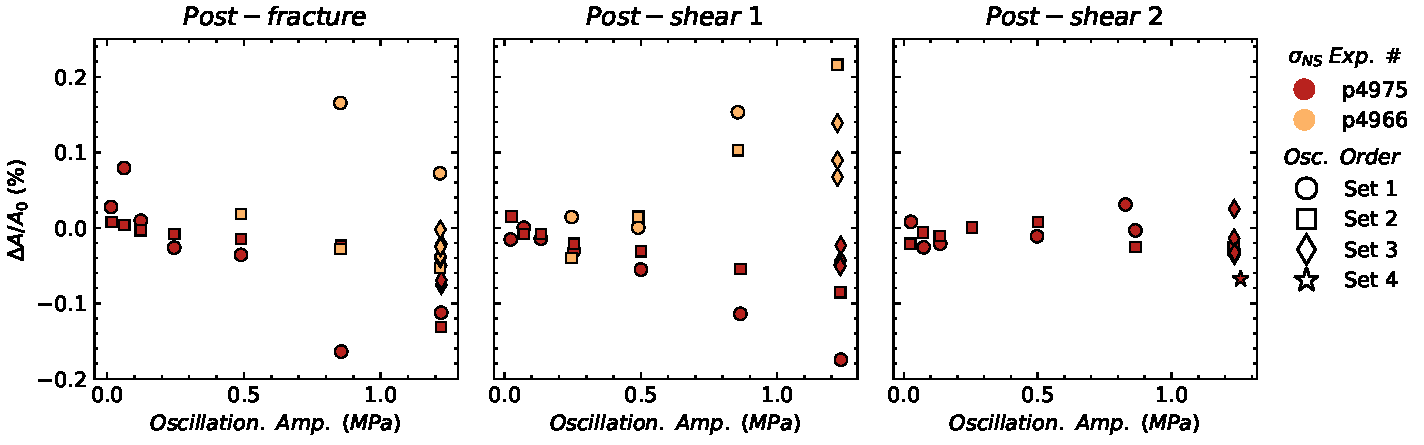
\includegraphics[width=1\columnwidth]{delA_amp_NS}
	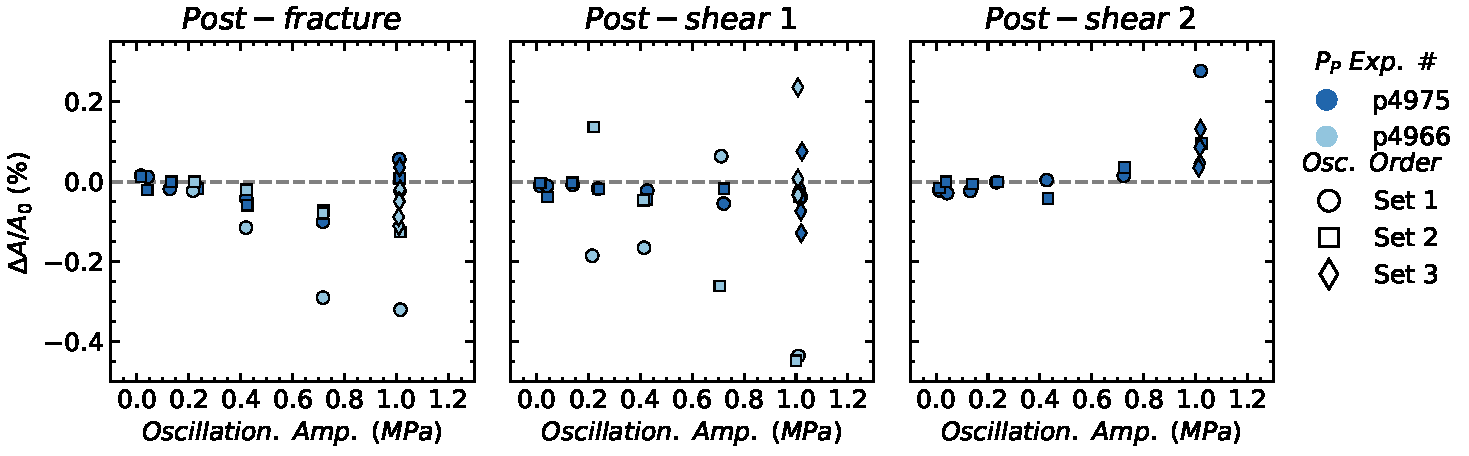
\includegraphics[width=1\columnwidth]{delA_amp_PP}
	%\enspace
	%\includegraphics[width=6cm]{post-frac_amp_array}
	\caption{RMS amplitude for direct-path receiver as a function of permeability change for $ \sigma_{NS} $ and $ P_P $ oscillations. Data point shapes oscillation order.  RMS amplitude decreases with oscillation amplitude and show little variation with order for experiment p4975. }
	\label{fig:delA_ns_amp}
\end{figure*}

\clearpage


\begin{figure*}[ht]
	\centering
	\includegraphics[width=1\columnwidth]{avg_DelA_perm_NS}
	\includegraphics[width=1\columnwidth]{avg_DelA_perm_PP}
	%\enspace
	%\includegraphics[width=6cm]{post-frac_amp_array}
	\caption{RMS amplitude averaged over all receivers as a function of permeability change for $ \sigma_{NS} $ and $ P_P $ oscillations. Data point shapes correspond to oscillation frequency and sizes to amplitude. There is a familiar trend that the average RMS amp. decreases with oscillation amplitude and frequency, except at high frequencies where there is anomalous behavior. Shearing the fracture weakens the relationship with relative permeability change.}
	\label{fig:dela_plots2}
\end{figure*}

\clearpage

\subsection{Velocity Amplitude Modulation during Oscillations}
\paragraph{}
The direct effect of dynamic stressing is an instantaneous modulation in wave velocity at harmonic frequencies of the driving frequency; we denote the mean velocity amplitude as $ dc $. The relative change in average velocity oscillations $ dc/c_0 $ is a proxy for the nonlinear parameter $ \beta $, estimated from the second harmonic (e.g., Rivière et al., 2013, 2015). We observe a monotonic relationship between the magnitude of $ dc/c_0 $ and oscillation amplitude for both rock samples (Figure \ref{fig:dc_plots2}). 

There is a consistent trend that subsequent oscillation sets decrease the magnitude of nonlinearity of $ dc/c_0 $ for Normal stress modulation. Pore pressure oscillations exhibit little to no change through subsequent repetitions, except for larger driving amplitudes.  

Shearing the fracture decreases, significantly for experiment p4966, the measured nonlinearity from Normal stress perturbations. This is also observed for Pore pressure oscillations in sample p4966, but p4975 exhibits little no change in $ dc/c_0 $ nonlinearity after the first shear. Then, after the second shear, Pore pressure oscillations interestingly increases the nonlinearity. We posit that the each dynamic stressing activate different mechanisms, likely resulting in the differences we observe. 
%Although the origins of $ \Delta c/c_0 $ and $ dc/c_0 $ remain unclear, there is empirical evidence that they stem from different micro-mechanical mechanisms (Rivière et al., 2016, 2015). \\



%Many rock types exhibit strongly nonlinear mesoscopic elastic (NME) behavior, such that the stiffness is highly strain-dependent for strains greater than ~$ 10^{-6} $ (Guyer \& Johnson, 2009). The presence of fractures increases the local compliance and thus enhances elastic nonlinearity. The nonlinearity of a fractured interface is dictated by the surface roughness and fracture stress (e.g., Jin et al., 2018). One of the elastodynamic signatures of NME materials is the strain-dependency of elastic wave velocity (see
% Figures 2c and 2d). The strain-induced changes in wave velocity ($ \Delta c/c_0 $ and $ dc/c_0 $ ) would be null for a perfectly linear elastic material because the elastic moduli in a linear elastic medium are constant and thus, the wave velocity is strain-invariant. However, in an NME material, the wave velocity drops instantaneously upon dynamic stressing. Our data support these statements. Our measurements of the relative changes in wave velocity $ \Delta c/c_0 $ show an initial sudden drop, which is known to be related to the hysteretic nonlinearity parameter $ \alpha $ (Guyer \& Johnson, 2009). This drop is followed by oscillatory fluctuations of wave velocity, which reach a non-equilibrium steady-state for sufficiently long perturbations (Rivière et al., 2015). The wave velocity oscillations occur primarily at the perturbation frequency ($ f $) but may also include higher order harmonics, $ nf $ for $ n = 2,3,... $ etc. The amplitude of velocity oscillations $ dc/c_0 $ (Figures 2c and 2d) is related to the nonlinear parameter $ \beta $ that is typically estimated via the second harmonic (e.g., Rivière et al., 2013, 2015). Once the perturbation ceases, the wave velocity slowly relaxes to the pre-oscillation value $ c_0 $ -- a phenomenon known as slow dynamics (TenCate et al., 2000; Shokouhi et al., 2017).

%A linear dependency is also apparent in dry intact Berea sandstone (Riviere et al., 2015). In addition, there is no discernible dependency on the frequency of oscillations. This observation aligns with that reported in a previous study (Riviere et al., 2016), where dc/c0 or the second harmonic amplitude was observed to be independent of the imposed oscillation frequency. 
%
%\begin{itemize}
%	\item Although the origins of $dc/c_0 $ and $ dc/c $ remain unclear, consider empirical evidence from [Rivière et al., 2015, 2016] that they originate from different micro-scale mechanisms 
%\end{itemize}

\clearpage

\begin{figure*}[ht]
	\centering
	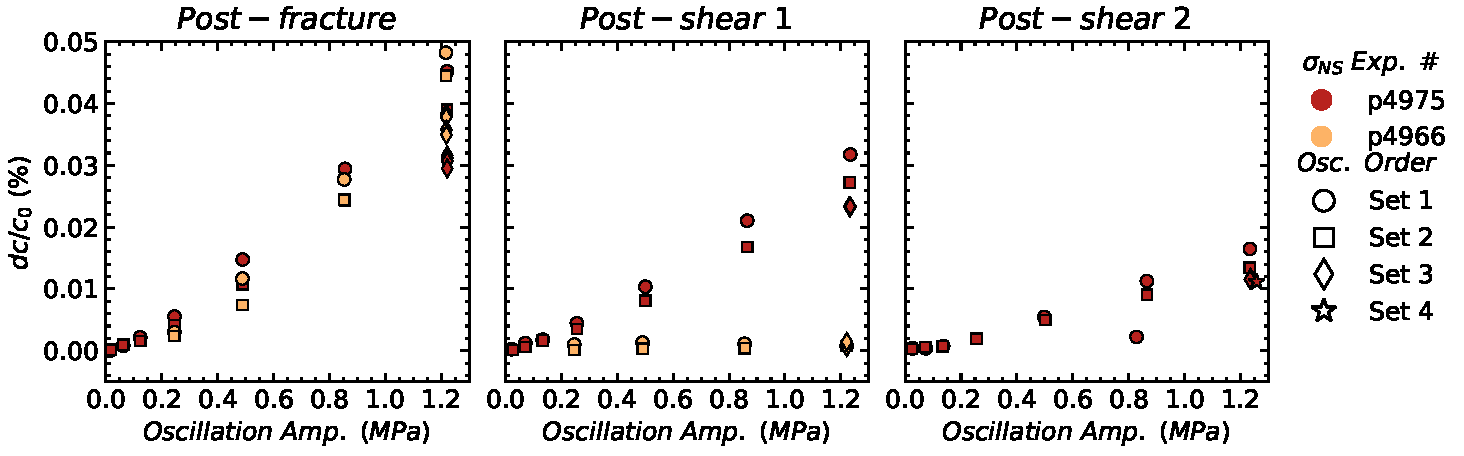
\includegraphics[width=1\columnwidth]{dc_amp_NS}
	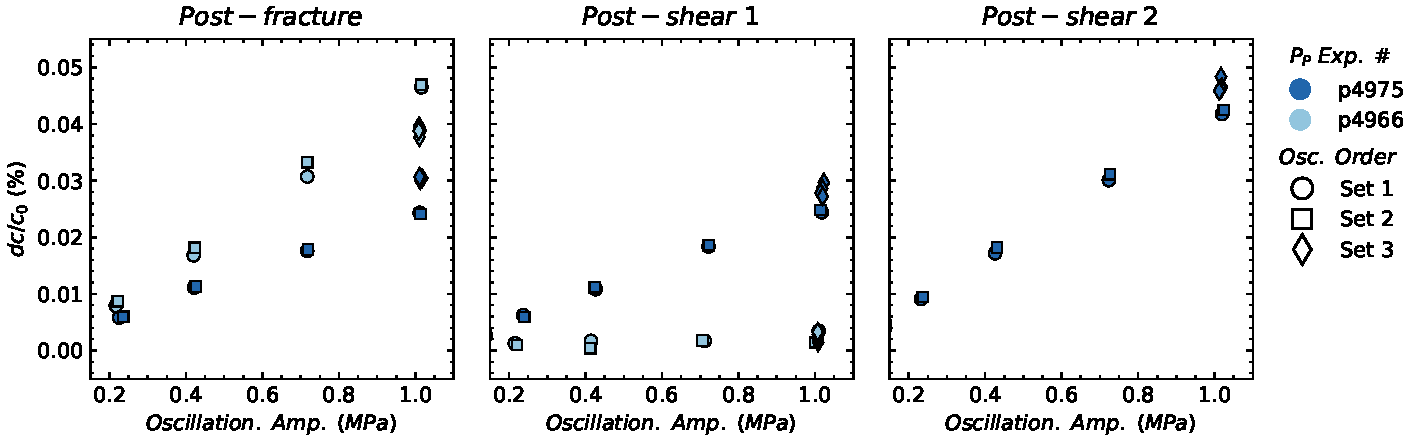
\includegraphics[width=1\columnwidth]{dc_amp_PP}
	%\enspace
	%\includegraphics[width=6cm]{post-frac_amp_array}
	\caption{Velocity amplitude modulation averaged over all receivers ($ dc/c_0 $) as a function of Normal stress and Pore pressure oscillations.}
	\label{fig:dc_plots2}
\end{figure*}

%\newpage

%\subsection{Recovery of Velocity and Permeability}
%\begin{itemize}
%	\item Although the origins of $ \Delta c/c_0 $ and $ dc/c $ remain unclear, consider empirical evidence from [Rivière et al., 2015, 2016] that they originate from different micro-scale mechanisms 
%\end{itemize}
%
%
%\begin{figure}[ht]
%	\centering
%%	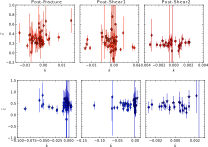
\includegraphics[width=1\columnwidth]{avgRecovBoth_NSPP}
%	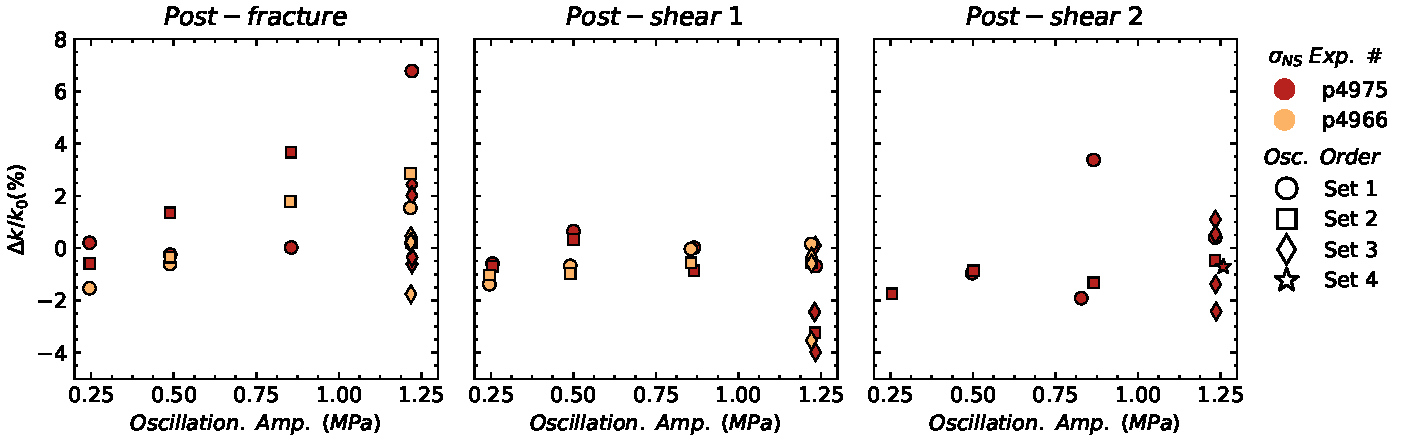
\includegraphics[width=1\columnwidth]{delk_amp_NS}
%	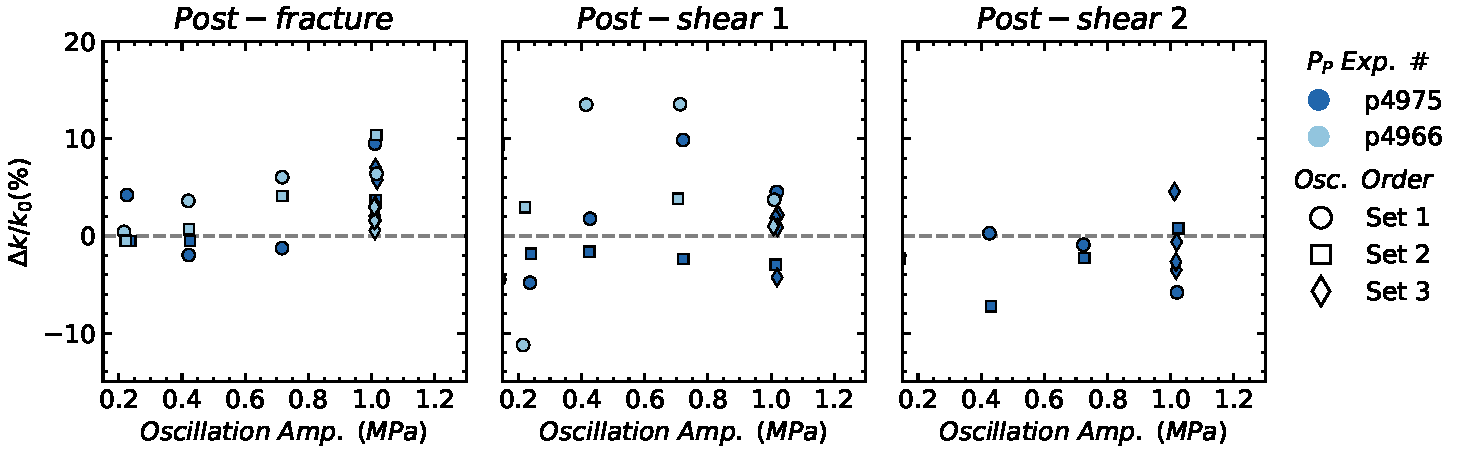
\includegraphics[width=1\columnwidth]{delk_amp_PP}
%	%\enspace
%	%\includegraphics[width=6cm]{post-frac_amp_array}
%	\caption{Velocity recovery averaged over all receivers ($ \overline {\dot c} $) as a function of oscillation amplitude for NS and PP oscillations. 
%	I suspect that the we are not waiting long enough to see a trend like J. Elkhoury and others. His recovery values were ~0.5, which he says is related to the dimensionality of the fracture. Shearing the fracture increases the complexity and maybe changes the slope -- dominated by clogging/moving wear material rather than mated aperture.}
%	\label{fig:cdot_amp}
%\end{figure}
%
%\newpage


%\begin{figure}[ht]
%	\centering
%	%	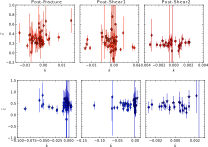
\includegraphics[width=1\columnwidth]{avgRecovBoth_NSPP}
%	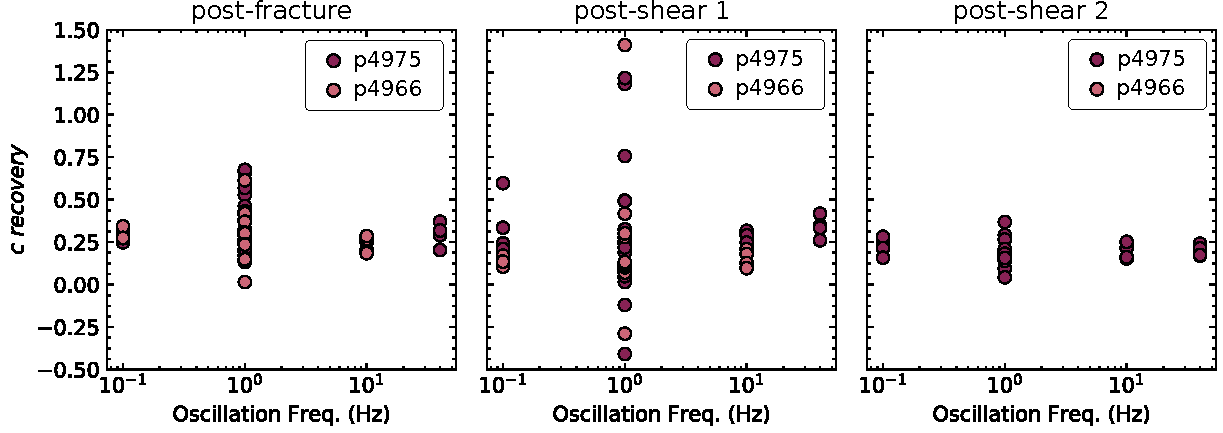
\includegraphics[width=1\columnwidth]{Cdot_NS_freq}
%	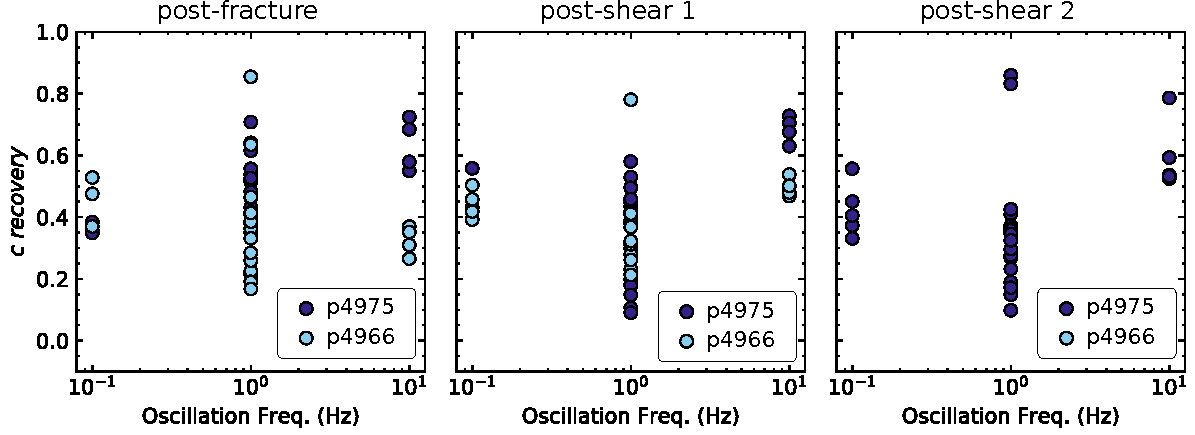
\includegraphics[width=1\columnwidth]{Cdot_PP_freq}
%	%\enspace
%	%\includegraphics[width=6cm]{post-frac_amp_array}
%	\caption{Velocity recovery averaged over all receivers ($ \overline {\dot c} $) as a function of oscillation frequency for NS and PP oscillations. 
%		I suspect that the we are not waiting long enough to see a trend like J. Elkhoury and others. His recovery values were ~0.5, which he says is related to the dimensionality of the fracture. Shearing the fracture increases the complexity and maybe changes the slope -- dominated by clogging/moving wear material rather than mated aperture.}
%	\label{fig:cdot_amp}
%\end{figure}

%\newpage

%\subsection{Effect of Fracture Aperture}
%\begin{itemize}
%	\item effect of fracture aperture modulated by shearing the fractured samples in two 5mm increments, repeating the dynamic stressing protocols. Elucidates how changes in the aperture size distribution due to shearing and wear–alter the fracture stiffness and the stress-dependency.
%	\item shearing of the fracture reduces the nonlinearity measured during normal stress oscillations
%	\item oscillations become generally less effective in enhancing the fracture permeability.
%	\item the correlation between the nonlinearity and permeability change and sample thickness change is stronger for NS oscillations than Pp. 
%	\item There is no clear correlation between perm change and flow rate during oscillations, suggesting “unclogging” may not be the sole mechanism responsible for perm change due to Pp oscillations. 
%	\item However, we report nonlinearity after the second shear history: indicative of possible differences in mechanisms activated during the two modes of stressing.
%\end{itemize}
%
%\newpage

\newcommand{\beginsupplement}{%
%	\setcounter{table}{0}
%	\renewcommand{\thetable}{S\arabic{table}}%
	\setcounter{figure}{0}
	\renewcommand{\thefigure}{S\arabic{figure}}%
}

\beginsupplement
\section{Supplemental}

\begin{figure*}[ht]
	\centering
	%	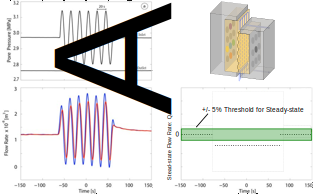
\includegraphics[width=1.0\columnwidth]{PpFlow_fig_v1}
	%	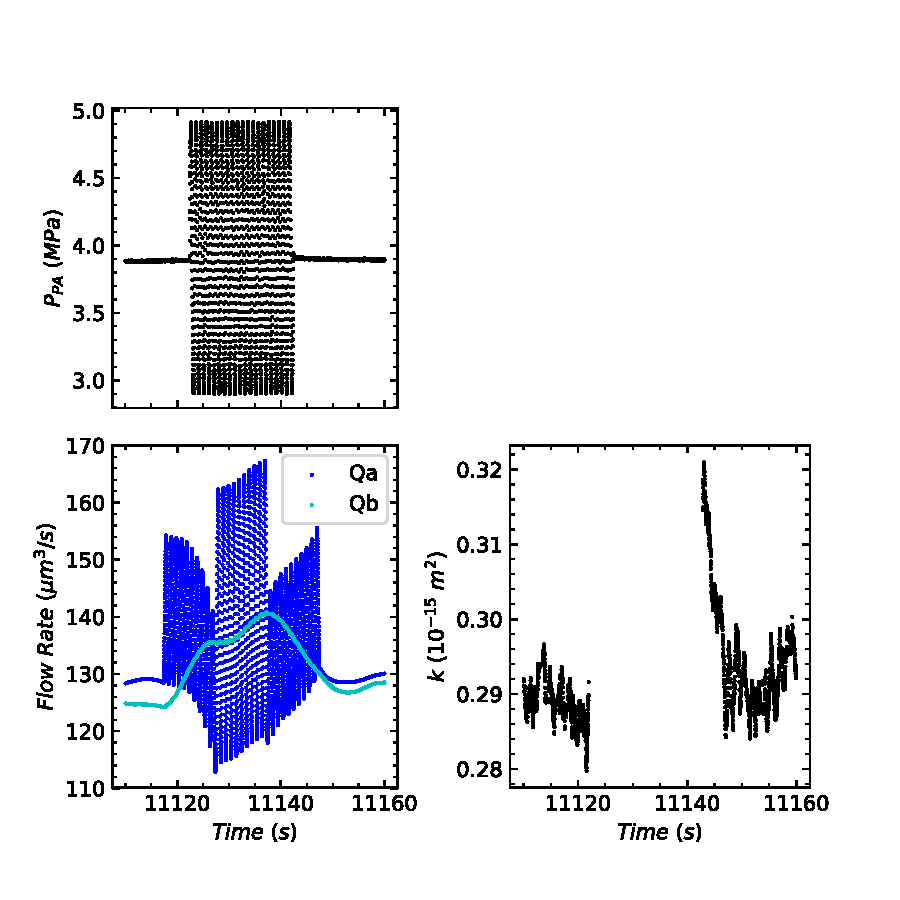
\includegraphics[width=0.8\columnwidth]{permCalcPlots_p4975_run3b_1Hz}
	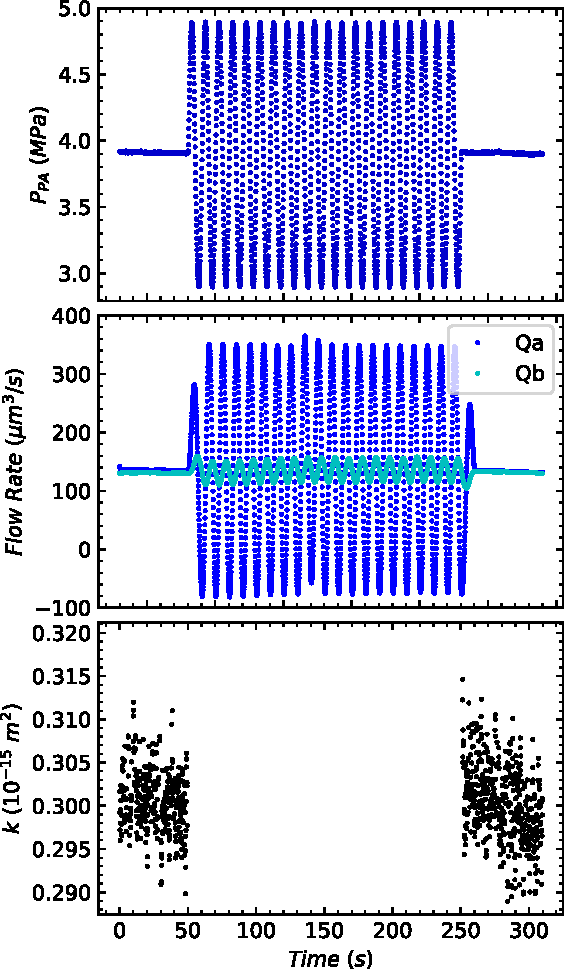
\includegraphics[width=0.4\columnwidth]{permCalcPlots_tall_p4975_run3b_1Hz}
	\caption[]{Example of dynamic stressing and the corresponding flow rate measurements for a set of pore pressure oscillations in experiment p4975. Note that the plots (a) and (b) are decimated for clarity. (a) Imposed pore pressure oscillation at inlet and fixed pore pressure at the outlet. Pressure conditions before and after the oscillations are identical. (b) Measured flow rates at the fracture inlet (blue line) and outlet (red dashed line). Notice the small time lag ($\leq$ 2 s) between the maxima of the inlet and outlet flow rates. (c) Permeability at steady-state and during the pore pressure oscillation. In the calculation of permeability we impose a threshold between the flow rates to ensure steady-state flow ($Q_{A} - Q_{B}  \leq 5 \% $). It is reasonable to assume that even at relatively low frequency oscillations, there is effectively no steady-state flow during the imposed oscillations.}
	\label{fig:perm_calc}
\end{figure*}

\textcolor{red}{We measure the effective permeability, ka, by calculating the flow rate over a 2 s window. For pore pressure oscillations, we start 10 s after the oscillation to ensure that permeability measurement is not affected by the Pp oscillation and/or by storage effects. Need to annotate Flow Rate with lines indicating the +- 5\%}

\newpage


%\begin{figure}[ht]
%	\centering
%	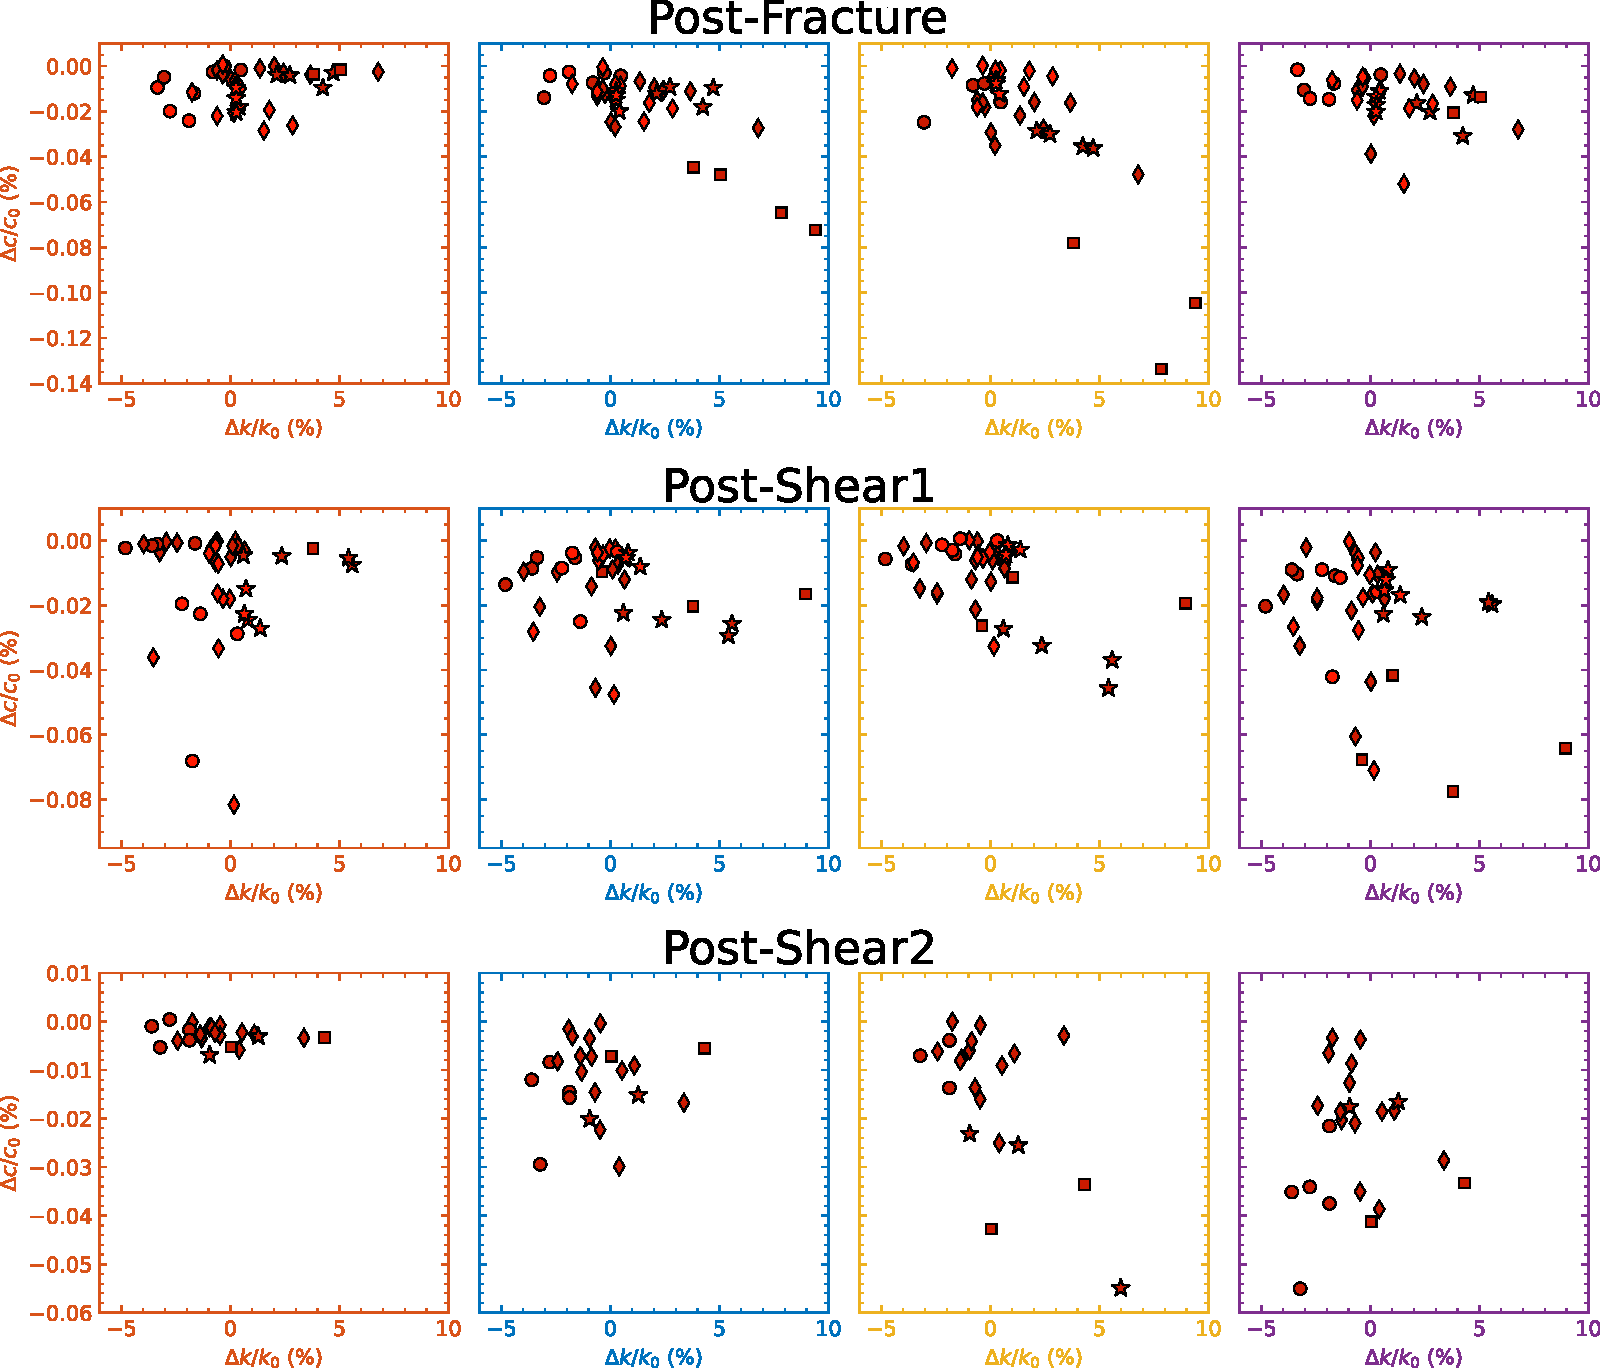
\includegraphics[width=1\columnwidth]{Delc_all_NS_all}
%	%\enspace
%	%\includegraphics[width=6cm]{post-frac_amp_array}
%	\caption{Nonlinearity as a function of permeability change for $ \sigma_{NS} $ oscillations for each receiver. Transitioning from post-fracture results to post-shear results, we observe decreased nonlinearity and permeability enhancement. This is probably related to clogging mechanisms.}%
%	\label{fig:delc_plots_ns}
%\end{figure}
%
%\newpage
%
%\begin{figure}[ht]
%	\centering
%	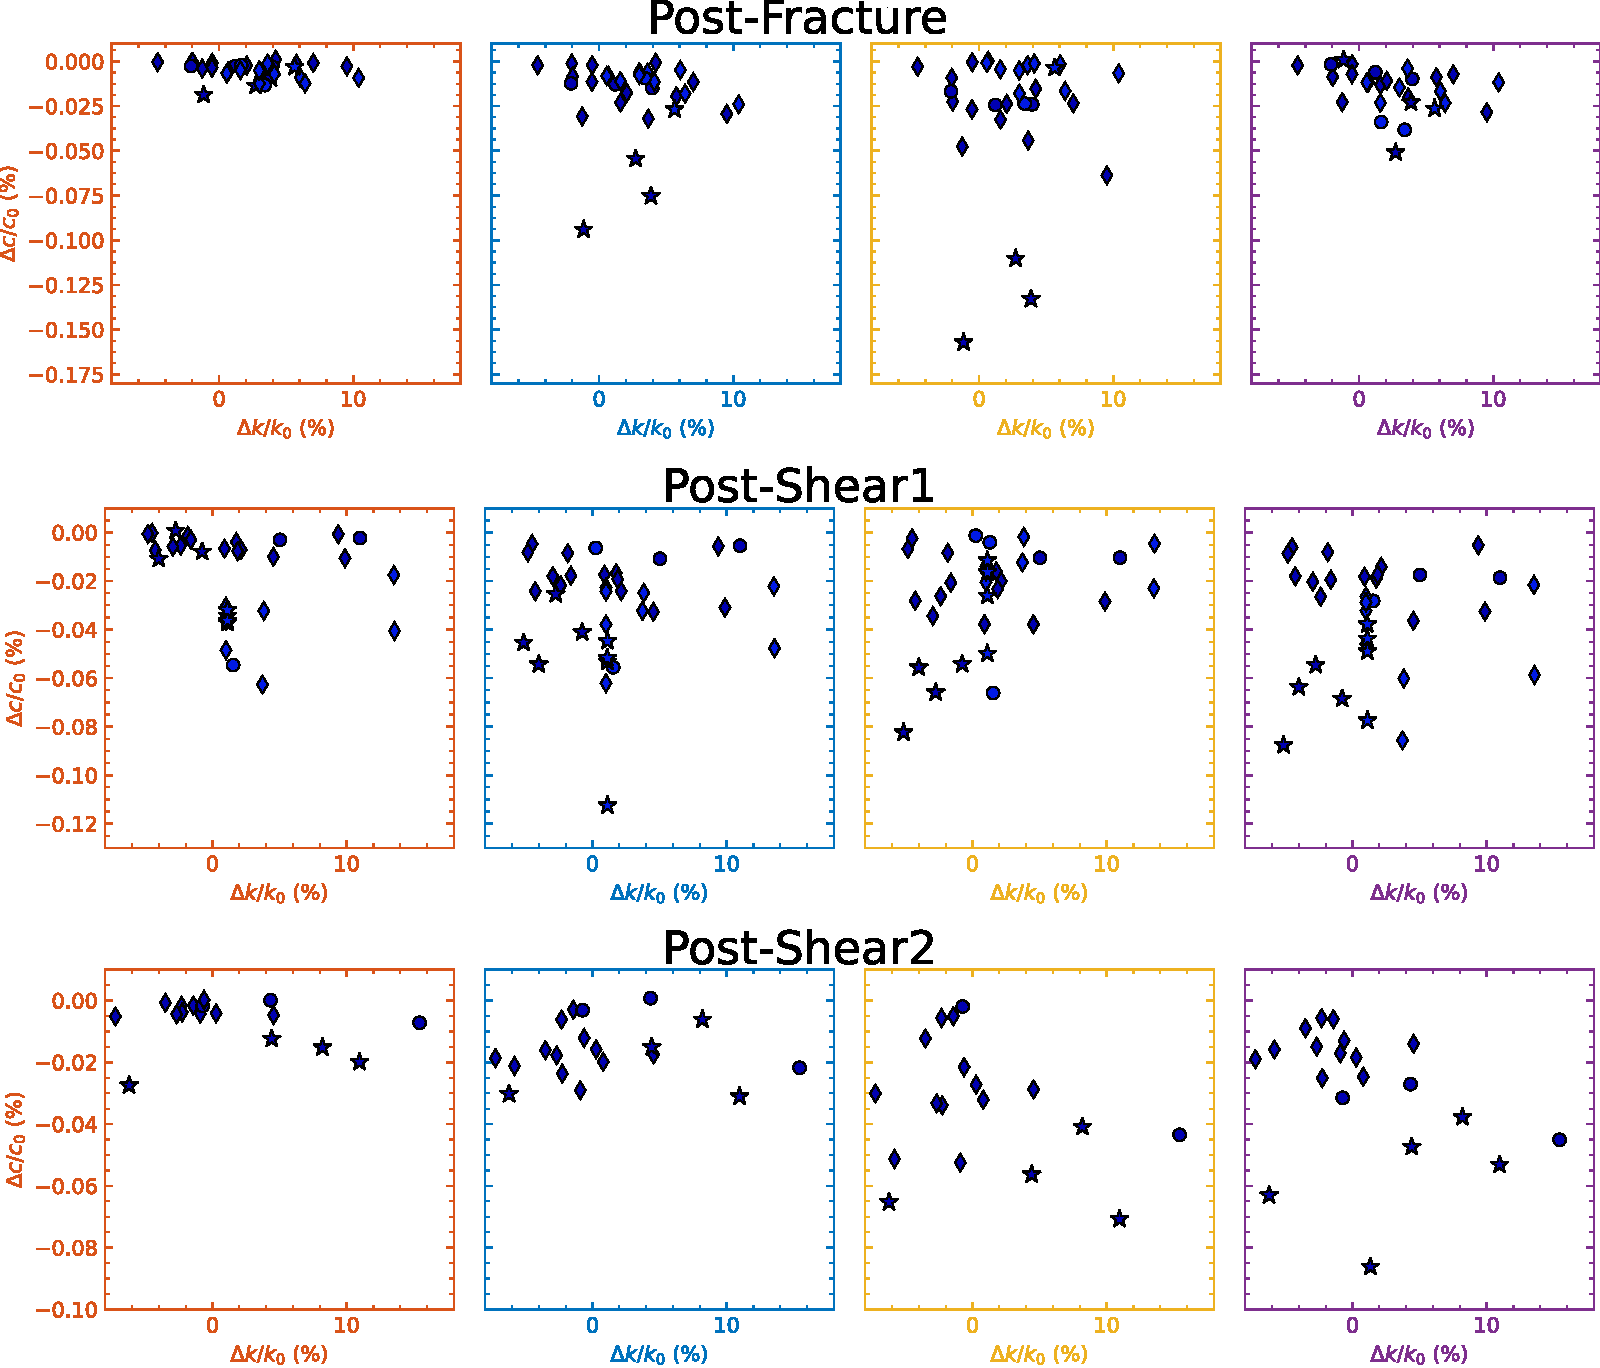
\includegraphics[width=1\columnwidth]{Delc_all_PP_all}
%	%\enspace
%	%\includegraphics[width=6cm]{post-frac_amp_array}
%	\caption{Nonlinearity as a function of permeability change for $ P_P $ oscillations for each receiver.}
%	\label{fig:delc_plots_pp}
%\end{figure}

\newpage

\begin{figure}[ht]
	\centering
	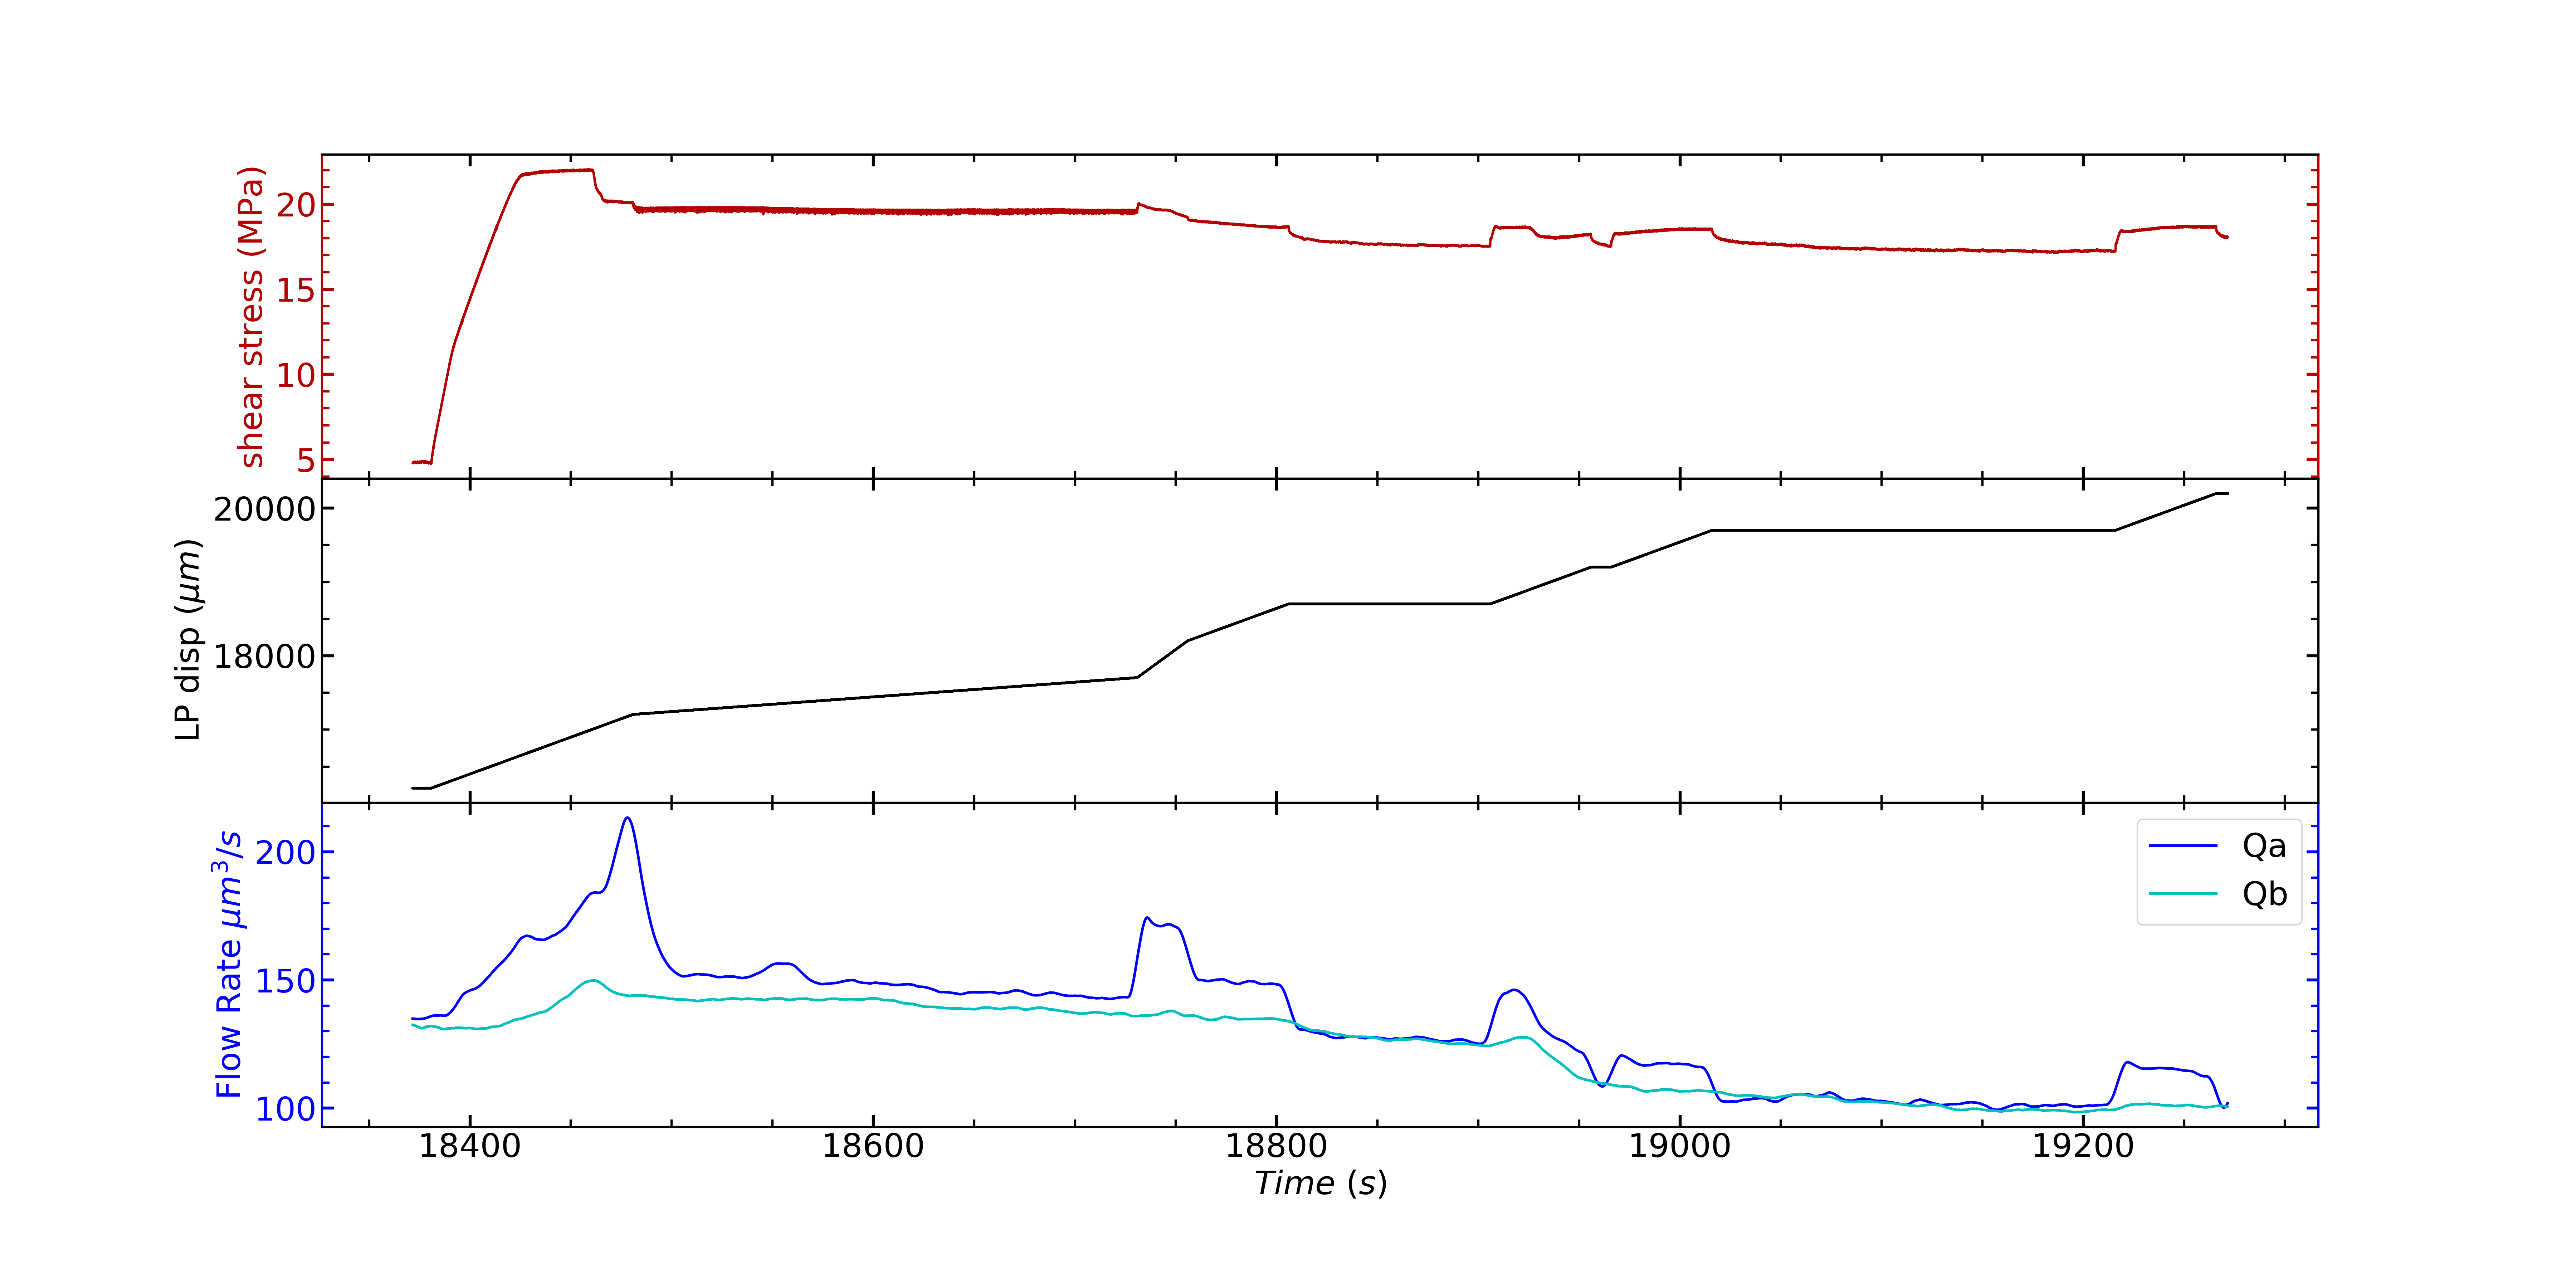
\includegraphics[width=1\columnwidth]{Shearing_p4975_shr1}
	\caption{First shearing for p4975.}
	\label{fig:shr1_p4975}
\end{figure}

\newpage

\begin{figure}[ht]
	\centering
	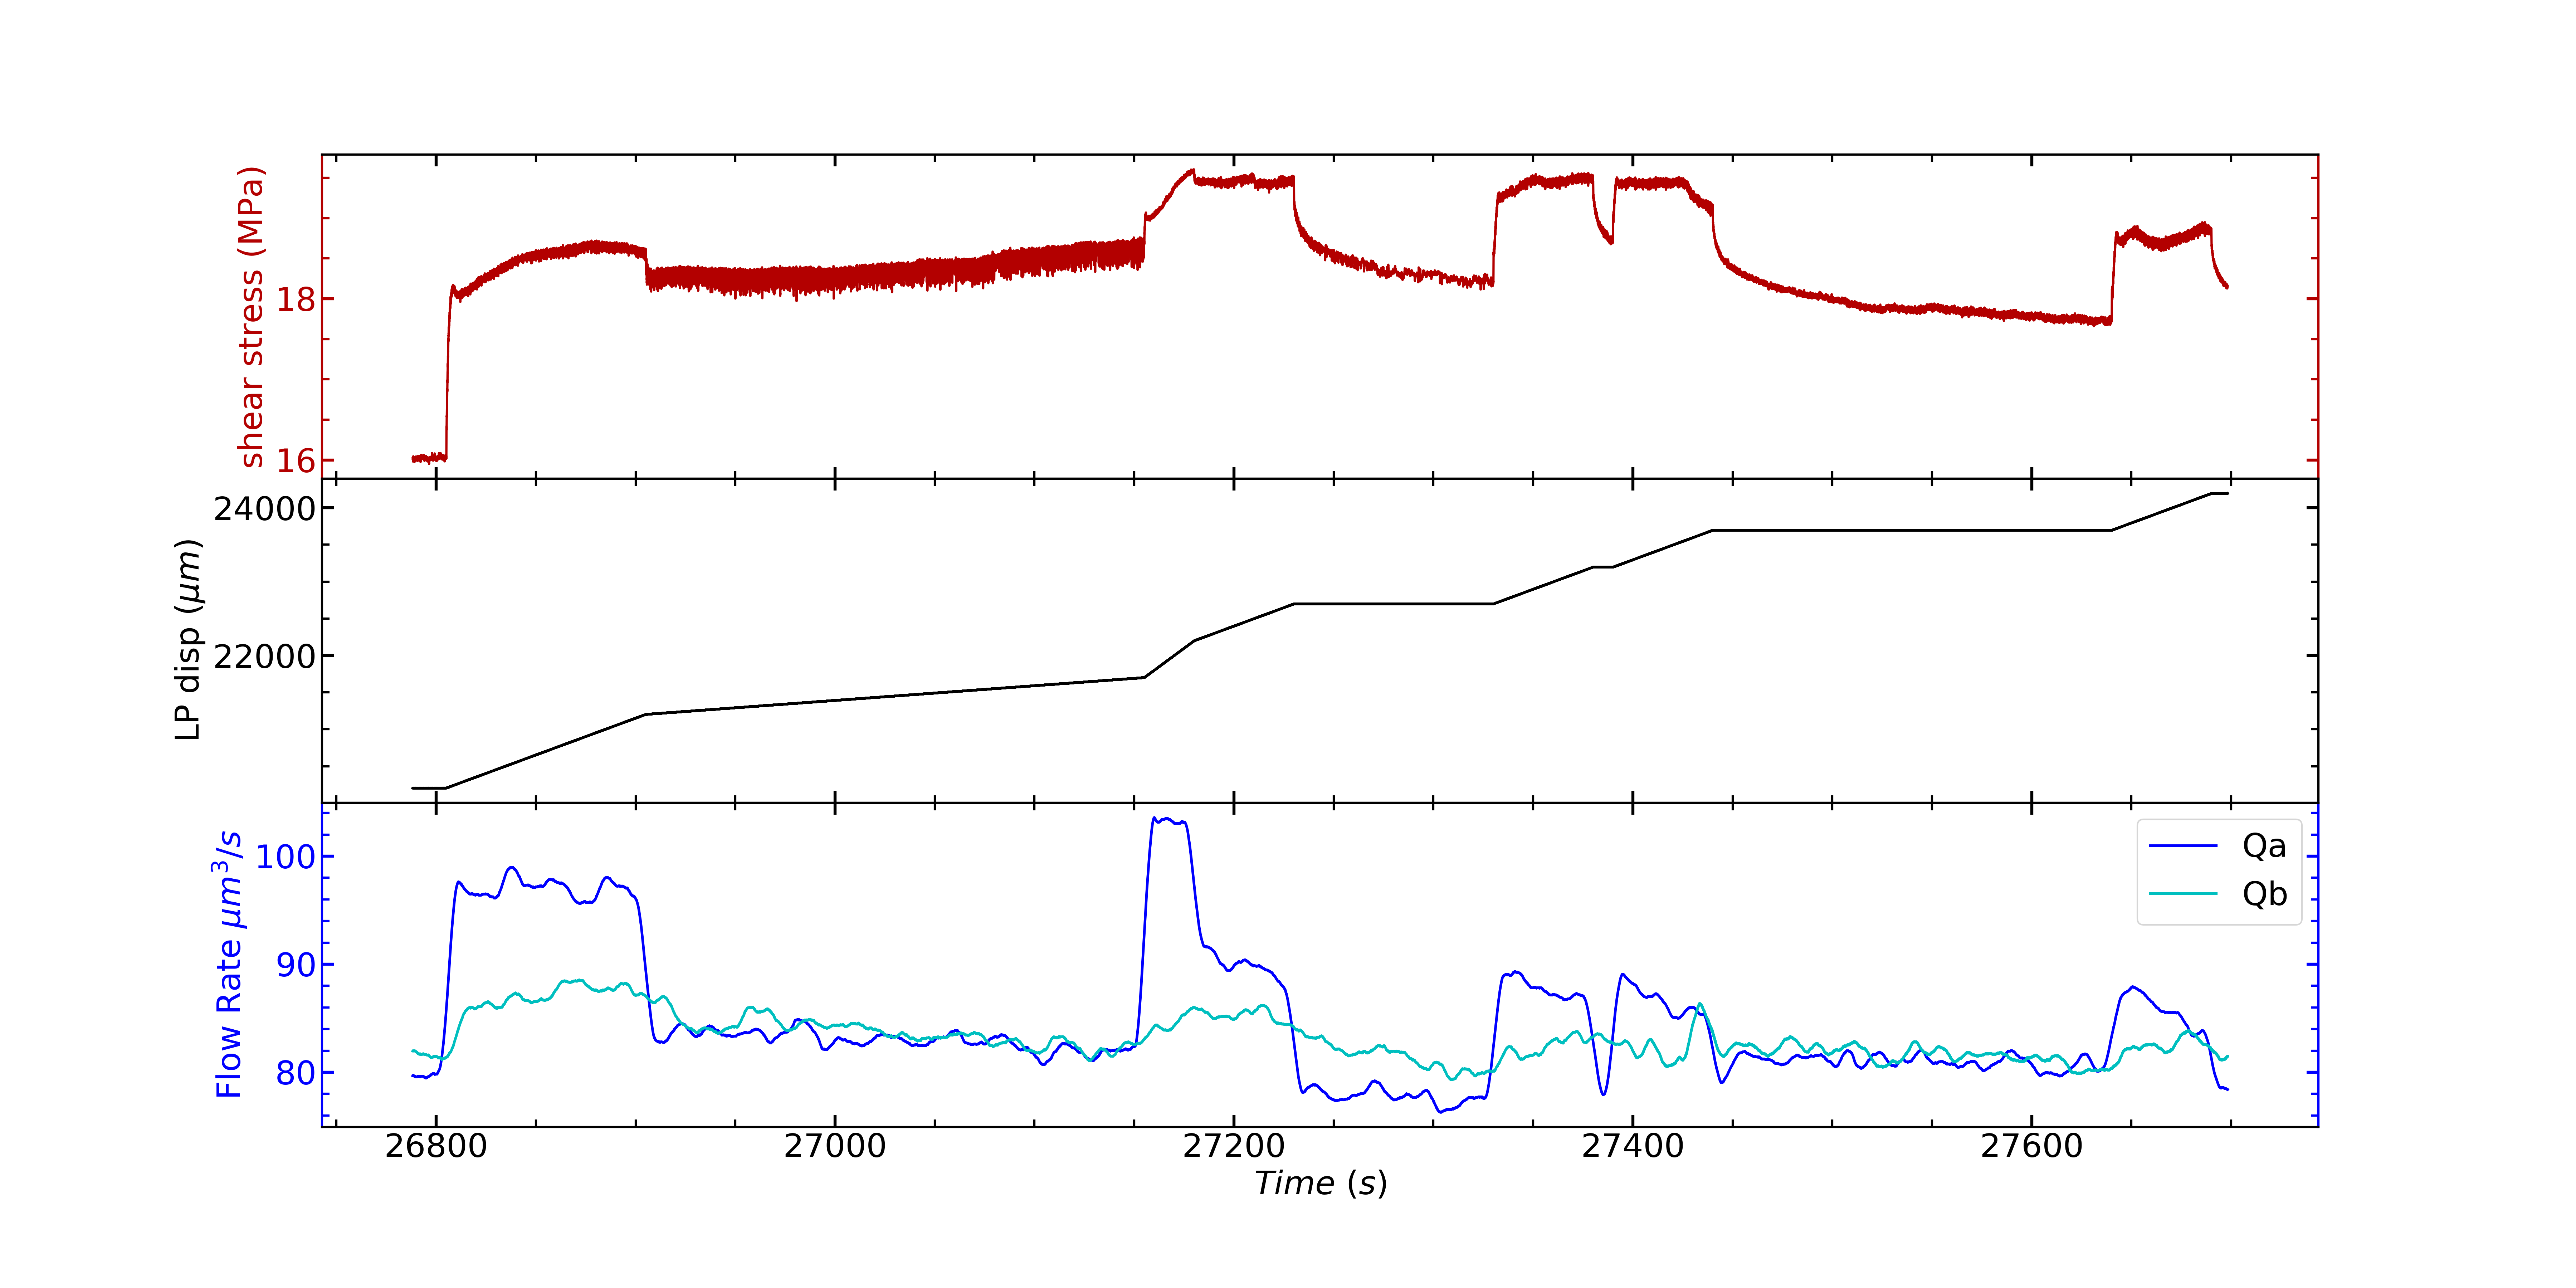
\includegraphics[width=1\columnwidth]{Shearing_p4975_shr2}
	\caption{Second shearing for p4975.}
	\label{fig:shr2_p4975}
\end{figure}

%++++++++++++++++++++++++++++++++++++++++
% References section will be created automatically 
% with inclusion of "thebibliography" environment
% as it shown below. See text starting with line
% \begin{thebibliography}{99}
% Note: with this approach it is YOUR responsibility to put them in order
% of appearance.

\bibliography{biblio_d13}
\bibliographystyle{ieeetr}

\end{document}